\section{A direct poset linked to Rational Dyck paths}

\subsection{Rational Dyck Paths}

\begin{definition}[a, b - Dyck path]
    An \emph{a, b - Dyck word} is a word $w \in \{0,1\}^*$
    such that :
    \begin{itemize}
        \item for each \emph{suffix} $w'$ of $w$,
            $$|w'|_1 \geqslant \frac{a}{b}|w'|_0$$.
        \item $|w|_0 = b$.
        \item $|w|_1 = a$.
    \end{itemize}
    An a, b - Dyck word can be represented as a 
    \emph{path} from $(0,0)$ to $(b,a)$ that stays over
    $y = \frac{a}{b}x$, called an \emph{a, b - Dyck path} :
    \begin{itemize}
        \item Each $1$ corresponds to a \emph{North step}
        $\uparrow$. 
        \item Each $0$ corresponds to an \emph{East step}
        $\rightarrow$.
    \end{itemize}
    We denote by $\mathcal{R}_{a, b}$ the set of
    a, b - Dyck words.
\end{definition}

\begin{example}[$a > b : a = 7, b = 3$]
    ~\\
    \begin{align*}
        &w_1 = 1110011110 \text{ is \emph{not} a 7, 3 - Dyck
        word, because } |11100|_1 = 3\\
        & \hspace{5cm} < \frac{7}{3}|11100|_0
        = \frac{14}{3} = 4 \frac{1}{3}.\\
        &w_2 = 1110111010 \text{ \emph{is} a 7, 3 - Dyck 
        word : }\\
    \end{align*}
    \begin{center}
        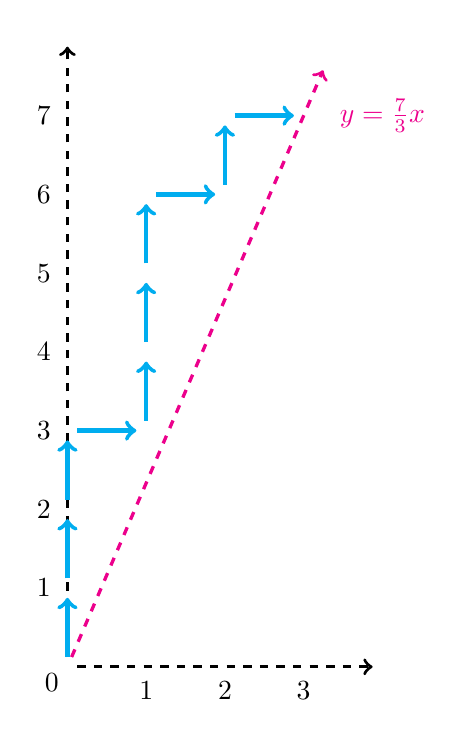
\begin{tikzpicture}[scale=1]
            \node (a) at (0, 0) {};
            \node (b) at (0, 8) {};
            \node (c) at (4, 0) {};
            \node (d) at (3.3, 7.7) {};
            \node (e) at (4, 7) [color = magenta]
                {$y = \frac{7}{3}x$}; 
            \draw [dashed, very thick, ->] (a) to (b);
            \draw [dashed, very thick, ->] (a) to (c);
            \draw [dashed, very thick, ->]
                [color = magenta] (a) to (d);

            \node (1)  at (0,0)   {};
            \node (2)  at (0,1)   {};
            \node (3)  at (0,2)   {};
            \node (4)  at (0,3)   {};
            \node (5)  at (1,3)   {};
            \node (6)  at (1,4)   {};
            \node (7)  at (1,5)   {};
            \node (8)  at (1,6)   {};
            \node (9)  at (2,6)   {};
            \node (10) at (2,7)   {};
            \node (11) at (3,7)   {};
            \draw [->, ultra thick, color = cyan]
                (1)  to (2);
            \draw [->, ultra thick, color = cyan] 
                (2)  to (3);
            \draw [->, ultra thick, color = cyan]
                (3)  to (4);
            \draw [->, ultra thick, color = cyan]
                (4)  to (5);
            \draw [->, ultra thick, color = cyan]
                (5)  to (6);
            \draw [->, ultra thick, color = cyan]
                (6)  to (7);
            \draw [->, ultra thick, color = cyan]
                (7)  to (8);
            \draw [->, ultra thick, color = cyan]
                (8)  to (9);
            \draw [->, ultra thick, color = cyan]
                (9)  to (10);
            \draw [->, ultra thick, color = cyan]
                (10) to (11);

            \node at (-0.2, -0.2) {$0$};
            \node at (-0.3, 1)    {$1$};
            \node at (1, -0.3)    {$1$};
            \node at (-0.3, 2)    {$2$};
            \node at (2, -0.3)    {$2$};
            \node at (-0.3, 3)    {$3$};
            \node at (3, -0.3)    {$3$};
            \node at (-0.3, 4)    {$4$};
            \node at (-0.3, 5)    {$5$};
            \node at (-0.3, 6)    {$6$};
            \node at (-0.3, 7)    {$7$};

        \end{tikzpicture}
    \end{center}
\end{example}

\begin{example}[$a < b : a = 3, b = 5$]
    ~\\
    \begin{align*}
        &w_1 = 10100010 \text{ is \emph{not} a 3, 5 - Dyck
        word, because } |101000|_1 = 2\\
        & \hspace{5cm} < \frac{3}{5}|101000|_0
        = \frac{12}{5} = 2 \frac{2}{5}.\\
        &w_2 = 10100100 \text{ \emph{is} a 3, 5 - Dyck 
        word : }\\
    \end{align*}
    \begin{center}
        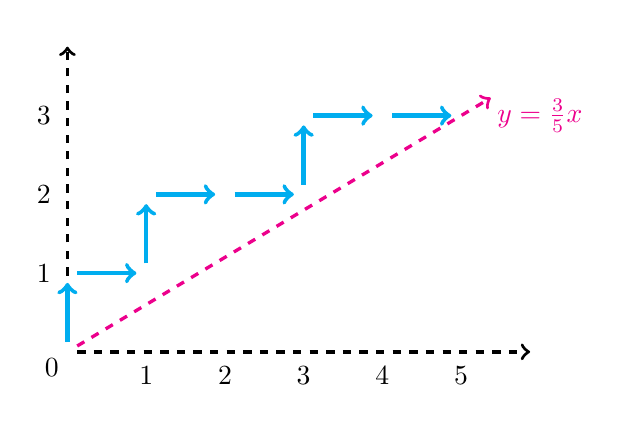
\begin{tikzpicture}[scale=1]
            \node (a) at (0, 0) {};
            \node (b) at (0, 4) {};
            \node (c) at (6, 0) {};
            \node (d) at (5.5, 3.3) {};
            \node (e) at (6, 3) [color = magenta]
                {$y = \frac{3}{5}x$}; 
            \draw [dashed, very thick, ->] (a) to (b);
            \draw [dashed, very thick, ->] (a) to (c);
            \draw [dashed, very thick, ->]
                [color = magenta] (a) to (d);

            \node (1)  at (0,0)   {};
            \node (2)  at (0,1)   {};
            \node (3)  at (1,1)   {};
            \node (4)  at (1,2)   {};
            \node (5)  at (2,2)   {};
            \node (6)  at (3,2)   {};
            \node (7)  at (3,3)   {};
            \node (8)  at (4,3)   {};
            \node (9)  at (5,3)   {};
            \draw [->, ultra thick, color = cyan]
                (1)  to (2);
            \draw [->, ultra thick, color = cyan] 
                (2)  to (3);
            \draw [->, ultra thick, color = cyan]
                (3)  to (4);
            \draw [->, ultra thick, color = cyan]
                (4)  to (5);
            \draw [->, ultra thick, color = cyan]
                (5)  to (6);
            \draw [->, ultra thick, color = cyan]
                (6)  to (7);
            \draw [->, ultra thick, color = cyan]
                (7)  to (8);
            \draw [->, ultra thick, color = cyan]
                (8)  to (9);

            \node at (-0.2, -0.2) {$0$};
            \node at (-0.3, 1)    {$1$};
            \node at (1, -0.3)    {$1$};
            \node at (-0.3, 2)    {$2$};
            \node at (2, -0.3)    {$2$};
            \node at (-0.3, 3)    {$3$};
            \node at (3, -0.3)    {$3$};
            \node at (4, -0.3)    {$4$};
            \node at (5, -0.3)    {$5$};

        \end{tikzpicture}
    \end{center}
\end{example}

\begin{theorem}
    Let $r_{a,b}$ be the cardinal of $\mathcal{R}_{a,b}$.
    We have $$r_{a,b} = \frac{1}{a+b} \binom {a+b}{a} =
    \frac{(a+b-1)!}{a!b!}$$, which is again the rational
    Catalan number.
\end{theorem}

\begin{example}[$a = 7, b = 2$]
    $r_n = 4$.
    \begin{center}
        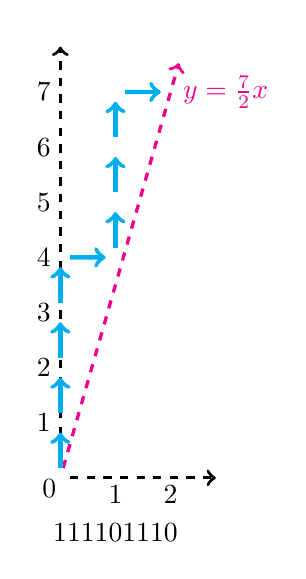
\begin{tikzpicture}[scale = 0.7]
            \node (a) at (0, 0) {};
            \node (b) at (0, 8) {};
            \node (c) at (3, 0) {};
            \node (d) at (2.2, 7.7) {};
            \node (e) at (3, 7) [color = magenta]
                {$y = \frac{7}{2}x$}; 
            \draw [dashed, very thick, ->] (a) to (b);
            \draw [dashed, very thick, ->] (a) to (c);
            \draw [dashed, very thick, ->]
                [color = magenta] (a) to (d);

            \node (1)  at (0,0)   {};
            \node (2)  at (0,1)   {};
            \node (3)  at (0,2)   {};
            \node (4)  at (0,3)   {};
            \node (5)  at (0,4)   {};
            \node (6)  at (1,4)   {};
            \node (7)  at (1,5)   {};
            \node (8)  at (1,6)   {};
            \node (9)  at (1,7)   {};
            \node (10) at (2,7)   {};
            \draw [->, ultra thick, color = cyan]
                (1)  to (2);
            \draw [->, ultra thick, color = cyan] 
                (2)  to (3);
            \draw [->, ultra thick, color = cyan]
                (3)  to (4);
            \draw [->, ultra thick, color = cyan]
                (4)  to (5);
            \draw [->, ultra thick, color = cyan]
                (5)  to (6);
            \draw [->, ultra thick, color = cyan]
                (6)  to (7);
            \draw [->, ultra thick, color = cyan]
                (7)  to (8);
            \draw [->, ultra thick, color = cyan]
                (8)  to (9);
            \draw [->, ultra thick, color = cyan]
                (9)  to (10);

            \node at (-0.2, -0.2) {$0$};
            \node at (-0.3, 1)    {$1$};
            \node at (1, -0.3)    {$1$};
            \node at (-0.3, 2)    {$2$};
            \node at (2, -0.3)    {$2$};
            \node at (-0.3, 3)    {$3$};
            \node at (-0.3, 4)    {$4$};
            \node at (-0.3, 5)    {$5$};
            \node at (-0.3, 6)    {$6$};
            \node at (-0.3, 7)    {$7$};
            \node at (1, -1)      {$111101110$};

        \end{tikzpicture}
        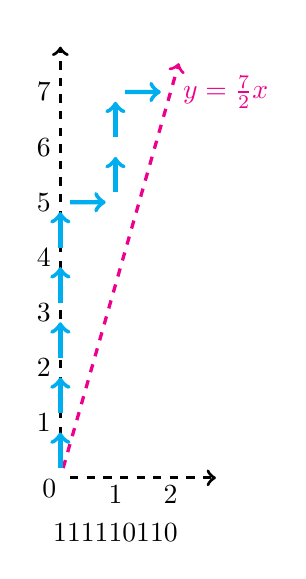
\begin{tikzpicture}[scale = 0.7]
            \node (a) at (0, 0) {};
            \node (b) at (0, 8) {};
            \node (c) at (3, 0) {};
            \node (d) at (2.2, 7.7) {};
            \node (e) at (3, 7) [color = magenta]
                {$y = \frac{7}{2}x$}; 
            \draw [dashed, very thick, ->] (a) to (b);
            \draw [dashed, very thick, ->] (a) to (c);
            \draw [dashed, very thick, ->]
                [color = magenta] (a) to (d);

            \node (1)  at (0,0)   {};
            \node (2)  at (0,1)   {};
            \node (3)  at (0,2)   {};
            \node (4)  at (0,3)   {};
            \node (5)  at (0,4)   {};
            \node (6)  at (0,5)   {};
            \node (7)  at (1,5)   {};
            \node (8)  at (1,6)   {};
            \node (9)  at (1,7)   {};
            \node (10) at (2,7)   {};
            \draw [->, ultra thick, color = cyan]
                (1)  to (2);
            \draw [->, ultra thick, color = cyan] 
                (2)  to (3);
            \draw [->, ultra thick, color = cyan]
                (3)  to (4);
            \draw [->, ultra thick, color = cyan]
                (4)  to (5);
            \draw [->, ultra thick, color = cyan]
                (5)  to (6);
            \draw [->, ultra thick, color = cyan]
                (6)  to (7);
            \draw [->, ultra thick, color = cyan]
                (7)  to (8);
            \draw [->, ultra thick, color = cyan]
                (8)  to (9);
            \draw [->, ultra thick, color = cyan]
                (9)  to (10);

            \node at (-0.2, -0.2) {$0$};
            \node at (-0.3, 1)    {$1$};
            \node at (1, -0.3)    {$1$};
            \node at (-0.3, 2)    {$2$};
            \node at (2, -0.3)    {$2$};
            \node at (-0.3, 3)    {$3$};
            \node at (-0.3, 4)    {$4$};
            \node at (-0.3, 5)    {$5$};
            \node at (-0.3, 6)    {$6$};
            \node at (-0.3, 7)    {$7$};
            \node at (1, -1)      {$111110110$};

        \end{tikzpicture}
        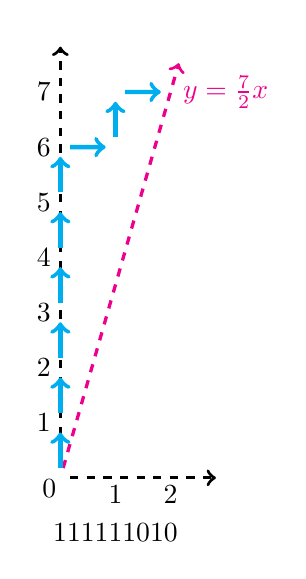
\begin{tikzpicture}[scale = 0.7]
            \node (a) at (0, 0) {};
            \node (b) at (0, 8) {};
            \node (c) at (3, 0) {};
            \node (d) at (2.2, 7.7) {};
            \node (e) at (3, 7) [color = magenta]
                {$y = \frac{7}{2}x$}; 
            \draw [dashed, very thick, ->] (a) to (b);
            \draw [dashed, very thick, ->] (a) to (c);
            \draw [dashed, very thick, ->]
                [color = magenta] (a) to (d);

            \node (1)  at (0,0)   {};
            \node (2)  at (0,1)   {};
            \node (3)  at (0,2)   {};
            \node (4)  at (0,3)   {};
            \node (5)  at (0,4)   {};
            \node (6)  at (0,5)   {};
            \node (7)  at (0,6)   {};
            \node (8)  at (1,6)   {};
            \node (9)  at (1,7)   {};
            \node (10) at (2,7)   {};
            \draw [->, ultra thick, color = cyan]
                (1)  to (2);
            \draw [->, ultra thick, color = cyan] 
                (2)  to (3);
            \draw [->, ultra thick, color = cyan]
                (3)  to (4);
            \draw [->, ultra thick, color = cyan]
                (4)  to (5);
            \draw [->, ultra thick, color = cyan]
                (5)  to (6);
            \draw [->, ultra thick, color = cyan]
                (6)  to (7);
            \draw [->, ultra thick, color = cyan]
                (7)  to (8);
            \draw [->, ultra thick, color = cyan]
                (8)  to (9);
            \draw [->, ultra thick, color = cyan]
                (9)  to (10);

            \node at (-0.2, -0.2) {$0$};
            \node at (-0.3, 1)    {$1$};
            \node at (1, -0.3)    {$1$};
            \node at (-0.3, 2)    {$2$};
            \node at (2, -0.3)    {$2$};
            \node at (-0.3, 3)    {$3$};
            \node at (-0.3, 4)    {$4$};
            \node at (-0.3, 5)    {$5$};
            \node at (-0.3, 6)    {$6$};
            \node at (-0.3, 7)    {$7$};
            \node at (1, -1)      {$111111010$};

        \end{tikzpicture}
        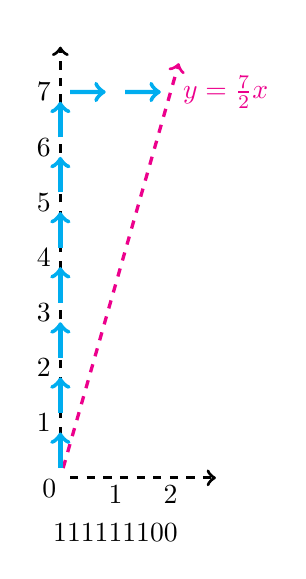
\begin{tikzpicture}[scale = 0.7]
            \node (a) at (0, 0) {};
            \node (b) at (0, 8) {};
            \node (c) at (3, 0) {};
            \node (d) at (2.2, 7.7) {};
            \node (e) at (3, 7) [color = magenta]
                {$y = \frac{7}{2}x$}; 
            \draw [dashed, very thick, ->] (a) to (b);
            \draw [dashed, very thick, ->] (a) to (c);
            \draw [dashed, very thick, ->]
                [color = magenta] (a) to (d);

            \node (1)  at (0,0)   {};
            \node (2)  at (0,1)   {};
            \node (3)  at (0,2)   {};
            \node (4)  at (0,3)   {};
            \node (5)  at (0,4)   {};
            \node (6)  at (0,5)   {};
            \node (7)  at (0,6)   {};
            \node (8)  at (0,7)   {};
            \node (9)  at (1,7)   {};
            \node (10) at (2,7)   {};
            \draw [->, ultra thick, color = cyan]
                (1)  to (2);
            \draw [->, ultra thick, color = cyan] 
                (2)  to (3);
            \draw [->, ultra thick, color = cyan]
                (3)  to (4);
            \draw [->, ultra thick, color = cyan]
                (4)  to (5);
            \draw [->, ultra thick, color = cyan]
                (5)  to (6);
            \draw [->, ultra thick, color = cyan]
                (6)  to (7);
            \draw [->, ultra thick, color = cyan]
                (7)  to (8);
            \draw [->, ultra thick, color = cyan]
                (8)  to (9);
            \draw [->, ultra thick, color = cyan]
                (9)  to (10);

            \node at (-0.2, -0.2) {$0$};
            \node at (-0.3, 1)    {$1$};
            \node at (1, -0.3)    {$1$};
            \node at (-0.3, 2)    {$2$};
            \node at (2, -0.3)    {$2$};
            \node at (-0.3, 3)    {$3$};
            \node at (-0.3, 4)    {$4$};
            \node at (-0.3, 5)    {$5$};
            \node at (-0.3, 6)    {$6$};
            \node at (-0.3, 7)    {$7$};
            \node at (1, -1)      {$111111100$};

        \end{tikzpicture}
    \end{center}
\end{example}

\begin{prop}
    This means we can create a \emph{bijection} between
    $\mathcal{PF'}_{a,b}$ and $\mathcal{R}_{a,b}$.
\end{prop}

\begin{proof}
    ~\
\begin{itemize}
    \item $\mathcal{PF'}_{a,b} \to \mathcal{R}_{a,b}$ :
    Let $f = (a_1, \ldots, a_n) \in \mathcal{PF'}_{a,b}$
    be our rational primitive parking function.
    For $i \in \{1, \ldots, b\}$, we define $l_i$ the
    number of occurences of $i$ in $f$.\\
    The corresponding rational Dyck word will be
    $\underbrace{1 \cdots 1}_{l_1}0
     \underbrace{1 \cdots 1}_{l_2}0 \cdots
     \underbrace{1 \cdots 1}_{l_b}0$.
    
    \item $\mathcal{R}_{a,b} \to \mathcal{PF'}_{a,b}$ :
    Let $w$ be our rational Dyck word, and consider its path
    representation. We define $s_i$ to be the distance
    between the segment from $(0, i - 1)$ to $(0, i)$
    and the $i^{th}$ North step. Then, let $a_i = s_i + 1$.\\
    The corresponding rational primitive parking function is 
    $(a_1, \ldots, a_a)$.
\end{itemize}
\end{proof}

\begin{rem}
    This bijection is exactly the same as the one between
    classical primitive parking functions and Dyck paths.
\end{rem}

\begin{example}[$a > b : a = 7, b = 3,
    \mathcal{PF'}_{a,b} \to \mathcal{R}_{a,b}$]
    ~\
    \begin{itemize}
        \item $f = (1, 1, 1, 2, 2, 3, 3)$
            \subitem $l_1 = 3$
            \hspace{2cm} $l_2 = 2$
            \hspace{2cm} $l_3 = 2$
        \item $w = (1110110110)$
    \end{itemize}

    \begin{center}
        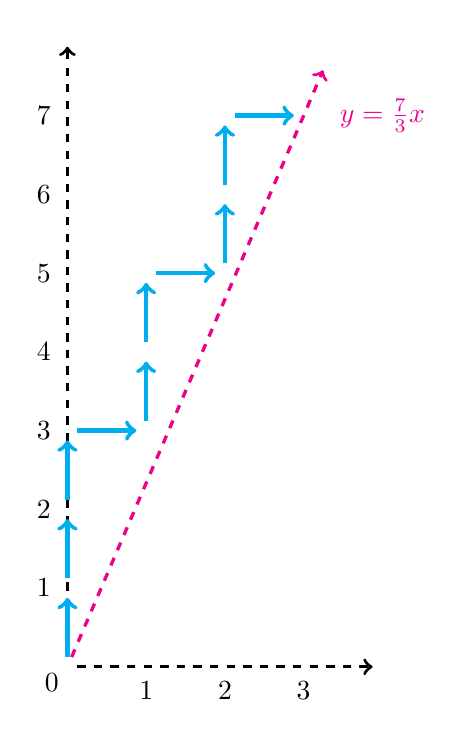
\begin{tikzpicture}[scale=1]
            \node (a) at (0, 0) {};
            \node (b) at (0, 8) {};
            \node (c) at (4, 0) {};
            \node (d) at (3.3, 7.7) {};
            \node (e) at (4, 7) [color = magenta]
                {$y = \frac{7}{3}x$}; 
            \draw [dashed, very thick, ->] (a) to (b);
            \draw [dashed, very thick, ->] (a) to (c);
            \draw [dashed, very thick, ->]
                [color = magenta] (a) to (d);

            \node (1)  at (0,0)   {};
            \node (2)  at (0,1)   {};
            \node (3)  at (0,2)   {};
            \node (4)  at (0,3)   {};
            \node (5)  at (1,3)   {};
            \node (6)  at (1,4)   {};
            \node (7)  at (1,5)   {};
            \node (8)  at (2,5)   {};
            \node (9)  at (2,6)   {};
            \node (10) at (2,7)   {};
            \node (11) at (3,7)   {};
            \draw [->, ultra thick, color = cyan]
                (1)  to (2);
            \draw [->, ultra thick, color = cyan] 
                (2)  to (3);
            \draw [->, ultra thick, color = cyan]
                (3)  to (4);
            \draw [->, ultra thick, color = cyan]
                (4)  to (5);
            \draw [->, ultra thick, color = cyan]
                (5)  to (6);
            \draw [->, ultra thick, color = cyan]
                (6)  to (7);
            \draw [->, ultra thick, color = cyan]
                (7)  to (8);
            \draw [->, ultra thick, color = cyan]
                (8)  to (9);
            \draw [->, ultra thick, color = cyan]
                (9)  to (10);
            \draw [->, ultra thick, color = cyan]
                (10) to (11);

            \node at (-0.2, -0.2) {$0$};
            \node at (-0.3, 1)    {$1$};
            \node at (1, -0.3)    {$1$};
            \node at (-0.3, 2)    {$2$};
            \node at (2, -0.3)    {$2$};
            \node at (-0.3, 3)    {$3$};
            \node at (3, -0.3)    {$3$};
            \node at (-0.3, 4)    {$4$};
            \node at (-0.3, 5)    {$5$};
            \node at (-0.3, 6)    {$6$};
            \node at (-0.3, 7)    {$7$};
        \end{tikzpicture}
    \end{center}
\end{example}

\begin{example}[$a < b : a = 3, b = 5,
    \mathcal{PF'}_{a,b} \to \mathcal{R}_{a,b}$]
    ~\
    \begin{itemize}
        \item $f = (1, 1, 4)$
            \subitem $l_1 = 2$
            \hspace{2cm} $l_2$
            \hspace{2cm} $l_3 = 0$
            \subitem $l_4 = 1$
            \hspace{2cm} $l_5 = 0$
        \item $w = 11000100$
    \end{itemize}

    \begin{center}
        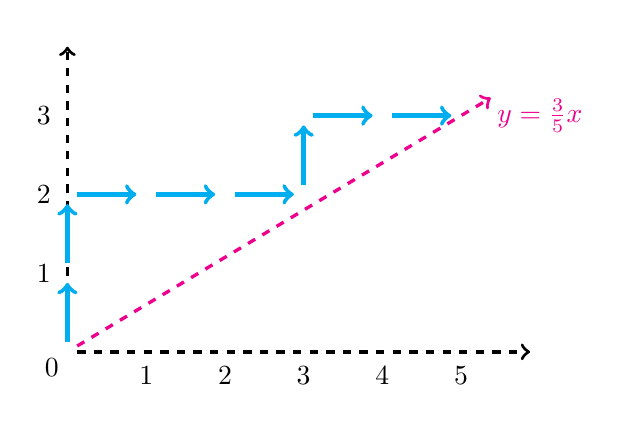
\begin{tikzpicture}[scale=1]
            \node (a) at (0, 0) {};
            \node (b) at (0, 4) {};
            \node (c) at (6, 0) {};
            \node (d) at (5.5, 3.3) {};
            \node (e) at (6, 3) [color = magenta]
                {$y = \frac{3}{5}x$}; 
            \draw [dashed, very thick, ->] (a) to (b);
            \draw [dashed, very thick, ->] (a) to (c);
            \draw [dashed, very thick, ->]
                [color = magenta] (a) to (d);

            \node (1)  at (0,0)   {};
            \node (2)  at (0,1)   {};
            \node (3)  at (0,2)   {};
            \node (4)  at (1,2)   {};
            \node (5)  at (2,2)   {};
            \node (6)  at (3,2)   {};
            \node (7)  at (3,3)   {};
            \node (8)  at (4,3)   {};
            \node (9)  at (5,3)   {};
            \draw [->, ultra thick, color = cyan]
                (1)  to (2);
            \draw [->, ultra thick, color = cyan] 
                (2)  to (3);
            \draw [->, ultra thick, color = cyan]
                (3)  to (4);
            \draw [->, ultra thick, color = cyan]
                (4)  to (5);
            \draw [->, ultra thick, color = cyan]
                (5)  to (6);
            \draw [->, ultra thick, color = cyan]
                (6)  to (7);
            \draw [->, ultra thick, color = cyan]
                (7)  to (8);
            \draw [->, ultra thick, color = cyan]
                (8)  to (9);

            \node at (-0.2, -0.2) {$0$};
            \node at (-0.3, 1)    {$1$};
            \node at (1, -0.3)    {$1$};
            \node at (-0.3, 2)    {$2$};
            \node at (2, -0.3)    {$2$};
            \node at (-0.3, 3)    {$3$};
            \node at (3, -0.3)    {$3$};
            \node at (4, -0.3)    {$4$};
            \node at (5, -0.3)    {$5$};
        \end{tikzpicture}
    \end{center}
\end{example}

\begin{example}[$a > b : a = 7, b = 3,
    \mathcal{R}_{a,b} \to \mathcal{PF'}_{a,b}$]
    ~\
    \begin{itemize}
        \item $w = 1111011010$
    \end{itemize}

    \begin{center}
        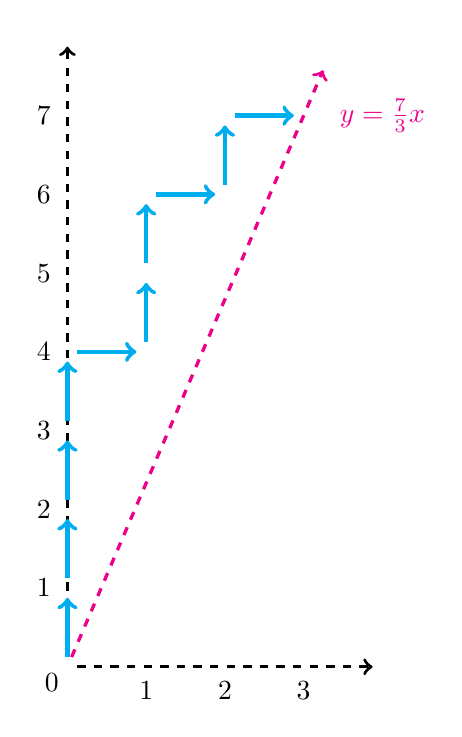
\begin{tikzpicture}[scale=1]
            \node (a) at (0, 0) {};
            \node (b) at (0, 8) {};
            \node (c) at (4, 0) {};
            \node (d) at (3.3, 7.7) {};
            \node (e) at (4, 7) [color = magenta]
                {$y = \frac{7}{3}x$}; 
            \draw [dashed, very thick, ->] (a) to (b);
            \draw [dashed, very thick, ->] (a) to (c);
            \draw [dashed, very thick, ->]
                [color = magenta] (a) to (d);

            \node (1)  at (0,0)   {};
            \node (2)  at (0,1)   {};
            \node (3)  at (0,2)   {};
            \node (4)  at (0,3)   {};
            \node (5)  at (0,4)   {};
            \node (6)  at (1,4)   {};
            \node (7)  at (1,5)   {};
            \node (8)  at (1,6)   {};
            \node (9)  at (2,6)   {};
            \node (10) at (2,7)   {};
            \node (11) at (3,7)   {};
            \draw [->, ultra thick, color = cyan]
                (1)  to (2);
            \draw [->, ultra thick, color = cyan] 
                (2)  to (3);
            \draw [->, ultra thick, color = cyan]
                (3)  to (4);
            \draw [->, ultra thick, color = cyan]
                (4)  to (5);
            \draw [->, ultra thick, color = cyan]
                (5)  to (6);
            \draw [->, ultra thick, color = cyan]
                (6)  to (7);
            \draw [->, ultra thick, color = cyan]
                (7)  to (8);
            \draw [->, ultra thick, color = cyan]
                (8)  to (9);
            \draw [->, ultra thick, color = cyan]
                (9)  to (10);
            \draw [->, ultra thick, color = cyan]
                (10) to (11);

            \node at (-0.2, -0.2) {$0$};
            \node at (-0.3, 1)    {$1$};
            \node at (1, -0.3)    {$1$};
            \node at (-0.3, 2)    {$2$};
            \node at (2, -0.3)    {$2$};
            \node at (-0.3, 3)    {$3$};
            \node at (3, -0.3)    {$3$};
            \node at (-0.3, 4)    {$4$};
            \node at (-0.3, 5)    {$5$};
            \node at (-0.3, 6)    {$6$};
            \node at (-0.3, 7)    {$7$};

        \end{tikzpicture}
    \end{center}
    \begin{itemize}
        \item Distances : 
            \subitem $s_1 = 0$
                \hspace{2cm} $a_1 = 1$
            \subitem $s_2 = 0$
                \hspace{2cm} $a_2 = 1$
            \subitem $s_3 = 0$
                \hspace{2cm} $a_3 = 1$
            \subitem $s_4 = 0$
                \hspace{2cm} $a_4 = 1$
            \subitem $s_5 = 1$
                \hspace{2cm} $a_5 = 2$
            \subitem $s_6 = 1$
                \hspace{2cm} $a_6 = 2$
            \subitem $s_7 = 2$
                \hspace{2cm} $a_7 = 3$
        \item $f = (1, 1, 1, 1, 2, 2, 3)$
    \end{itemize}
    
\end{example}

\begin{example}[$a < b : a = 3, b = 5,
    \mathcal{R}_{a,b} \to \mathcal{PF'}_{a,b}$]
    ~\
    \begin{itemize}
        \item $w = 10101000$
    \end{itemize}

    \begin{center}
        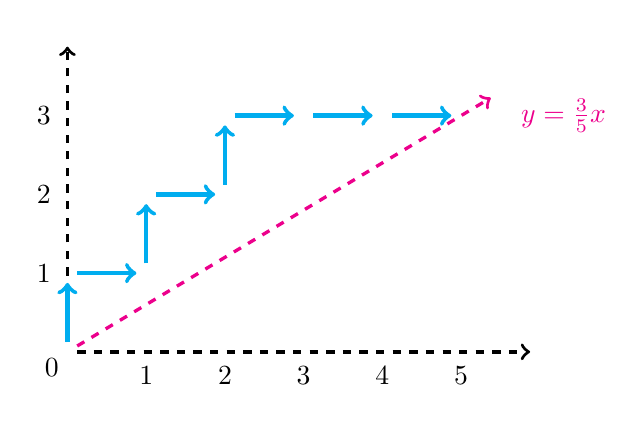
\begin{tikzpicture}[scale=1]
            \node (a) at (0, 0) {};
            \node (b) at (0, 4) {};
            \node (c) at (6, 0) {};
            \node (d) at (5.5, 3.3) {};
            \node (e) at (6.3, 3) [color = magenta]
                {$y = \frac{3}{5}x$}; 
            \draw [dashed, very thick, ->] (a) to (b);
            \draw [dashed, very thick, ->] (a) to (c);
            \draw [dashed, very thick, ->]
                [color = magenta] (a) to (d);

            \node (1)  at (0,0)   {};
            \node (2)  at (0,1)   {};
            \node (3)  at (1,1)   {};
            \node (4)  at (1,2)   {};
            \node (5)  at (2,2)   {};
            \node (6)  at (2,3)   {};
            \node (7)  at (3,3)   {};
            \node (8)  at (4,3)   {};
            \node (9)  at (5,3)   {};
            \draw [->, ultra thick, color = cyan]
                (1)  to (2);
            \draw [->, ultra thick, color = cyan] 
                (2)  to (3);
            \draw [->, ultra thick, color = cyan]
                (3)  to (4);
            \draw [->, ultra thick, color = cyan]
                (4)  to (5);
            \draw [->, ultra thick, color = cyan]
                (5)  to (6);
            \draw [->, ultra thick, color = cyan]
                (6)  to (7);
            \draw [->, ultra thick, color = cyan]
                (7)  to (8);
            \draw [->, ultra thick, color = cyan]
                (8)  to (9);

            \node at (-0.2, -0.2) {$0$};
            \node at (-0.3, 1)    {$1$};
            \node at (1, -0.3)    {$1$};
            \node at (-0.3, 2)    {$2$};
            \node at (2, -0.3)    {$2$};
            \node at (-0.3, 3)    {$3$};
            \node at (3, -0.3)    {$3$};
            \node at (4, -0.3)    {$4$};
            \node at (5, -0.3)    {$5$};

        \end{tikzpicture}
    \end{center}
    \begin{itemize}
        \item Distances : 
            \subitem $s_1 = 0$
                \hspace{2cm} $a_1 = 1$
            \subitem $s_2 = 1$
                \hspace{2cm} $a_2 = 2$
            \subitem $s_3 = 2$
                \hspace{2cm} $a_3 = 3$
        \item $f = (1, 2, 3)$
    \end{itemize}
    
\end{example}

\subsection{Rational Labeled Dyck Paths}

\begin{definition}[Labeled a, b - Dyck Path]
    A \emph{labeled a, b - Dyck word} is a word $w \in 
    \{0, \ldots, n\}^*$ such that :
    \begin{itemize}
        \item for each suffix $w'$ of $w$,
            $$|w'|_{\neq 0} \geqslant \frac{a}{b}|w'|_0$$.
        \item $|w|_0 = b$.
        \item $|w|_{\neq 0} = a$.
        \item for each $i \in \{1, \ldots, a\}$, $w$ has 
            exactly one occurence of $i$.
        \item if $w_i \neq 0$ and $w_{i+1} \neq 0$,
            then $w_i < w_{i+1}$. That is, consecutive
            North steps have increasing labels.
    \end{itemize}
    A labeled a, b - Dyck word can be represented
    as a path from $(0,0)$ to $(b,a)$, where each North
    step is associated to a label :
    \begin{itemize}
        \item Each $i \neq 0$ corresponds to a
            \emph{North step} $\uparrow$ labeled $i$.
        \item Each $0$ corresponds to an
            \emph{East step} $\rightarrow$.
    \end{itemize}
    Those paths are called \emph{labeled a, b - Dyck paths}.\\
    We denote by $\mathcal{LR}_{a,b}$ the set of labeled
    a, b - Dyck words.
\end{definition}

\begin{example}[$a > b : a = 7, b = 3$]
       $w_2 = 2456017030$ :\\
    \begin{center}
        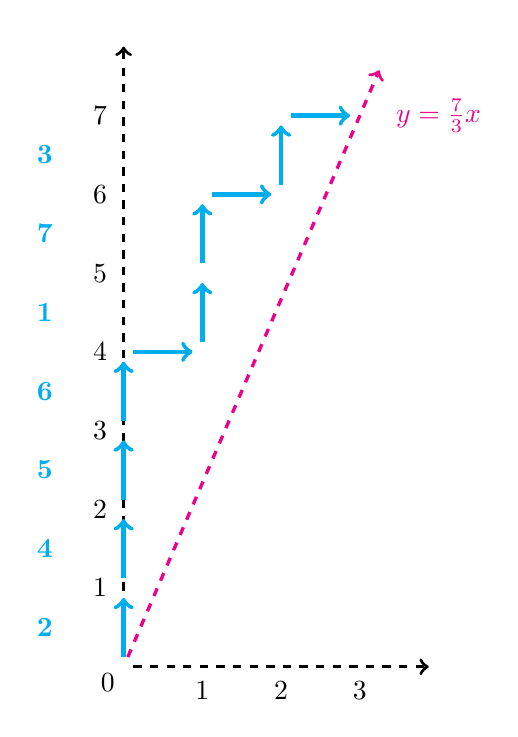
\begin{tikzpicture}[scale=1]
            \node (a) at (0, 0) {};
            \node (b) at (0, 8) {};
            \node (c) at (4, 0) {};
            \node (d) at (3.3, 7.7) {};
            \node (e) at (4, 7) [color = magenta]
                {$y = \frac{7}{3}x$}; 
            \draw [dashed, very thick, ->] (a) to (b);
            \draw [dashed, very thick, ->] (a) to (c);
            \draw [dashed, very thick, ->]
                [color = magenta] (a) to (d);

            \node (1)  at (0,0)   {};
            \node (2)  at (0,1)   {};
            \node (3)  at (0,2)   {};
            \node (4)  at (0,3)   {};
            \node (5)  at (0,4)   {};
            \node (6)  at (1,4)   {};
            \node (7)  at (1,5)   {};
            \node (8)  at (1,6)   {};
            \node (9)  at (2,6)   {};
            \node (10) at (2,7)   {};
            \node (11) at (3,7)   {};
            \draw [->, ultra thick, color = cyan]
                (1)  to (2);
            \draw [->, ultra thick, color = cyan] 
                (2)  to (3);
            \draw [->, ultra thick, color = cyan]
                (3)  to (4);
            \draw [->, ultra thick, color = cyan]
                (4)  to (5);
            \draw [->, ultra thick, color = cyan]
                (5)  to (6);
            \draw [->, ultra thick, color = cyan]
                (6)  to (7);
            \draw [->, ultra thick, color = cyan]
                (7)  to (8);
            \draw [->, ultra thick, color = cyan]
                (8)  to (9);
            \draw [->, ultra thick, color = cyan]
                (9)  to (10);
            \draw [->, ultra thick, color = cyan]
                (10) to (11);

            \node at (-0.2, -0.2) {$0$};
            \node at (-0.3, 1)    {$1$};
            \node at (1, -0.3)    {$1$};
            \node at (-0.3, 2)    {$2$};
            \node at (2, -0.3)    {$2$};
            \node at (-0.3, 3)    {$3$};
            \node at (3, -0.3)    {$3$};
            \node at (-0.3, 4)    {$4$};
            \node at (-0.3, 5)    {$5$};
            \node at (-0.3, 6)    {$6$};
            \node at (-0.3, 7)    {$7$};

            \node [color = cyan] at (-1, 0.5) {\textbf{2}};
            \node [color = cyan] at (-1, 1.5) {\textbf{4}};
            \node [color = cyan] at (-1, 2.5) {\textbf{5}};
            \node [color = cyan] at (-1, 3.5) {\textbf{6}};
            \node [color = cyan] at (-1, 4.5) {\textbf{1}};
            \node [color = cyan] at (-1, 5.5) {\textbf{7}};
            \node [color = cyan] at (-1, 6.5) {\textbf{3}};
        \end{tikzpicture}
    \end{center}
\end{example}

\begin{example}[$a < b : a = 3, b = 5$]
    $w = 20130000$ :\\
 \begin{center}
     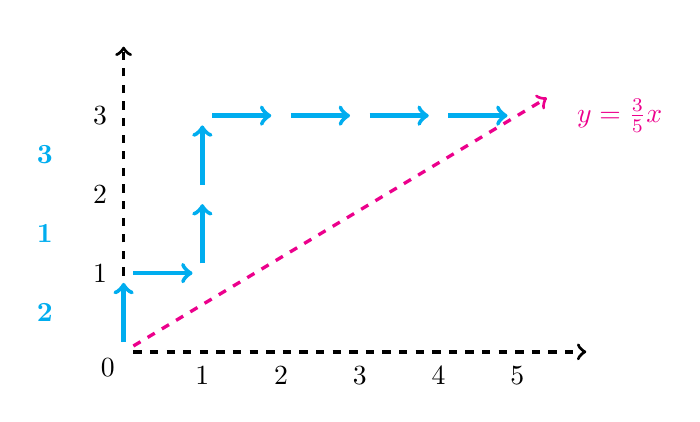
\begin{tikzpicture}[scale=1]
         \node (a) at (0, 0) {};
         \node (b) at (0, 4) {};
         \node (c) at (6, 0) {};
         \node (d) at (5.5, 3.3) {};
         \node (e) at (6.3, 3) [color = magenta]
             {$y = \frac{3}{5}x$}; 
         \draw [dashed, very thick, ->] (a) to (b);
         \draw [dashed, very thick, ->] (a) to (c);
         \draw [dashed, very thick, ->]
             [color = magenta] (a) to (d);

         \node (1)  at (0,0)   {};
         \node (2)  at (0,1)   {};
         \node (3)  at (1,1)   {};
         \node (4)  at (1,2)   {};
         \node (5)  at (1,3)   {};
         \node (6)  at (2,3)   {};
         \node (7)  at (3,3)   {};
         \node (8)  at (4,3)   {};
         \node (9)  at (5,3)   {};
         \draw [->, ultra thick, color = cyan]
             (1)  to (2);
         \draw [->, ultra thick, color = cyan] 
             (2)  to (3);
         \draw [->, ultra thick, color = cyan]
             (3)  to (4);
         \draw [->, ultra thick, color = cyan]
             (4)  to (5);
         \draw [->, ultra thick, color = cyan]
             (5)  to (6);
         \draw [->, ultra thick, color = cyan]
             (6)  to (7);
         \draw [->, ultra thick, color = cyan]
             (7)  to (8);
         \draw [->, ultra thick, color = cyan]
             (8)  to (9);

         \node at (-0.2, -0.2) {$0$};
         \node at (-0.3, 1)    {$1$};
         \node at (1, -0.3)    {$1$};
         \node at (-0.3, 2)    {$2$};
         \node at (2, -0.3)    {$2$};
         \node at (-0.3, 3)    {$3$};
         \node at (3, -0.3)    {$3$};
         \node at (4, -0.3)    {$4$};
         \node at (5, -0.3)    {$5$};

         \node [color = cyan] at (-1, 0.5) {\textbf{2}};
         \node [color = cyan] at (-1, 1.5) {\textbf{1}};
         \node [color = cyan] at (-1, 2.5) {\textbf{3}};
     \end{tikzpicture}
 \end{center}
\end{example}

\begin{theorem}
    Let $lr_{a,b}$ be the cardinal of $\mathcal{LR}_{a,b}$.
    We have $$lr_{a,b} = b^{a - 1}$$.
\end{theorem}

\begin{example}[$a > b : a = 4, b = 3$]
    $lr_{a,b} = 3^3 = 27$
    \begin{itemize}
        \item Word of shape $XXXX000$ :
            \subitem $1234000$
        \item Words of shape $XXX0X00$ :
            \subitem $1230400$
            \hspace{2cm} $1240300$
            \hspace{2cm} $1340200$
            \subitem $2340100$
        \item Words of shape $XX0XX00$ :
            \subitem $1203400$
            \hspace{2cm} $1302400$
            \hspace{2cm} $1402300$
            \subitem $2301400$
            \hspace{2cm} $2401300$
            \hspace{2cm} $3401200$
        \item Words of shape $XXX00X0$ :
            \subitem $1230040$
            \hspace{2cm} $1240030$
            \hspace{2cm} $1340020$
            \subitem $2340010$
        \item Words of shape $XX0X0X0$ :
            \subitem $1203040$
            \hspace{2cm} $1204030$
            \hspace{2cm} $1302040$
            \subitem $1304020$
            \hspace{2cm} $1402030$
            \hspace{2cm} $1403020$
            \subitem $2301040$
            \hspace{2cm} $2304010$
            \hspace{2cm} $2401030$
            \subitem $2403010$
            \hspace{2cm} $3401020$
            \hspace{2cm} $3402010$
    \end{itemize}
    
\end{example}

\begin{prop}
    This means we can create a \emph{bijection} between
    $\mathcal{PF}_{a,b}$ and $\mathcal{LR}_{a,b}$.
\end{prop}

\begin{proof}
    ~\
    \begin{itemize}
        \item $\mathcal{PF}_{a,b} \to \mathcal{LR}_{a,b}$ :
        Let $f = (a_1, \ldots, a_n) \in \mathcal{PF}_{a,b}$
        be our a, b - parking function. For $i \in \{1, \ldots,
        b\}$, we define $im_i$ : $\{j\ |\ a_j = i\}$. \\
        We then define $im_{i,1}, \ldots, im_{i,k_i}$ to be
        the elements of $im_i$ in increasing order.\\
        The corresponding labeled a, b - Dyck word will be \\
        $\underbrace{im_{1,1} \cdots im_{1,k_1}}_{im_1}0
         \underbrace{im_{2,1} \cdots im_{2,k_2}}_{im_2}0
         \cdots
         \underbrace{im_{n,1} \cdots im_{b,k_b}}_{im_b}0$.

        \item $\mathcal{LR}_{a,b} \to \mathcal{PF}_n$ :
        Let w be our labeled a, b - Dyck word, and consider its
        path representation. We define $s_i$ to be the
        distance between the segment from $(0, i-1)$ to
        $(0,i)$ and the $i^{th}$ North step.\\
        Then, let $label(i)$ be the label of the $i^{th}$
        North step, and $dist_i = \{label(j) | s_j = i\}$
        be the set of the labels of all North steps at
        distance $i$.\\
        Then, if $j \in dist_i$, let $a_j = i + 1$.\\
        The corresponding parking function is
        $(a_1, \ldots, a_a)$.
    \end{itemize}
\end{proof}

\begin{rem}
    This bijection is exactly the same as the one between
    classical parking functions and labeled Dyck paths.
\end{rem}

\begin{example}[$a > b : a = 7, b = 3,
        \mathcal{PF}_{a,b} \to \mathcal{LR}_{a,b}$]
    ~\
    \begin{itemize}
        \item $f = (2, 1, 3, 1, 1, 3, 2)$
            \subitem $im_1 = \{2, 4, 5\}$
            \hspace{16mm} $im_2 = \{1, 7\}$
            \hspace{24mm} $im_3 = \{3, 6\}$
        \item $w = 2450170360$
    \end{itemize}
    \begin{center}
        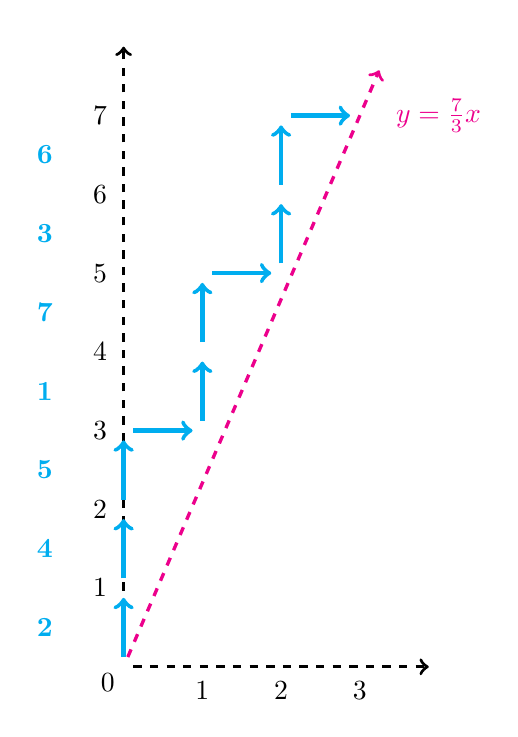
\begin{tikzpicture}[scale=1]
            \node (a) at (0, 0) {};
            \node (b) at (0, 8) {};
            \node (c) at (4, 0) {};
            \node (d) at (3.3, 7.7) {};
            \node (e) at (4, 7) [color = magenta]
                {$y = \frac{7}{3}x$}; 
            \draw [dashed, very thick, ->] (a) to (b);
            \draw [dashed, very thick, ->] (a) to (c);
            \draw [dashed, very thick, ->]
                [color = magenta] (a) to (d);

            \node (1)  at (0,0)   {};
            \node (2)  at (0,1)   {};
            \node (3)  at (0,2)   {};
            \node (4)  at (0,3)   {};
            \node (5)  at (1,3)   {};
            \node (6)  at (1,4)   {};
            \node (7)  at (1,5)   {};
            \node (8)  at (2,5)   {};
            \node (9)  at (2,6)   {};
            \node (10) at (2,7)   {};
            \node (11) at (3,7)   {};
            \draw [->, ultra thick, color = cyan]
                (1)  to (2);
            \draw [->, ultra thick, color = cyan] 
                (2)  to (3);
            \draw [->, ultra thick, color = cyan]
                (3)  to (4);
            \draw [->, ultra thick, color = cyan]
                (4)  to (5);
            \draw [->, ultra thick, color = cyan]
                (5)  to (6);
            \draw [->, ultra thick, color = cyan]
                (6)  to (7);
            \draw [->, ultra thick, color = cyan]
                (7)  to (8);
            \draw [->, ultra thick, color = cyan]
                (8)  to (9);
            \draw [->, ultra thick, color = cyan]
                (9)  to (10);
            \draw [->, ultra thick, color = cyan]
                (10) to (11);

            \node at (-0.2, -0.2) {$0$};
            \node at (-0.3, 1)    {$1$};
            \node at (1, -0.3)    {$1$};
            \node at (-0.3, 2)    {$2$};
            \node at (2, -0.3)    {$2$};
            \node at (-0.3, 3)    {$3$};
            \node at (3, -0.3)    {$3$};
            \node at (-0.3, 4)    {$4$};;
            \node at (-0.3, 5)    {$5$};
            \node at (-0.3, 6)    {$6$};
            \node at (-0.3, 7)    {$7$};

            \node [color = cyan] at (-1, 0.5) {\textbf{2}};
            \node [color = cyan] at (-1, 1.5) {\textbf{4}};
            \node [color = cyan] at (-1, 2.5) {\textbf{5}};
            \node [color = cyan] at (-1, 3.5) {\textbf{1}};
            \node [color = cyan] at (-1, 4.5) {\textbf{7}};
            \node [color = cyan] at (-1, 5.5) {\textbf{3}};
            \node [color = cyan] at (-1, 6.5) {\textbf{6}};

        \end{tikzpicture}
    \end{center}
\end{example}

\begin{example}[$a < b : a = 3, b = 5,
    \mathcal{PF}_{a,b} \to \mathcal{LR}_{a,b}$]
~\
\begin{itemize}
    \item $f = (4, 1, 2)$
        \subitem $im_1 = \{2\}$
        \hspace{16mm} $im_2 = \{3\}$
        \hspace{24mm} $im_3 = \emptyset$
        \subitem $im_4 = \{1\}$
        \hspace{16mm} $im_5 = \emptyset$
    \item $w = 20300100$
\end{itemize}
\begin{center}
    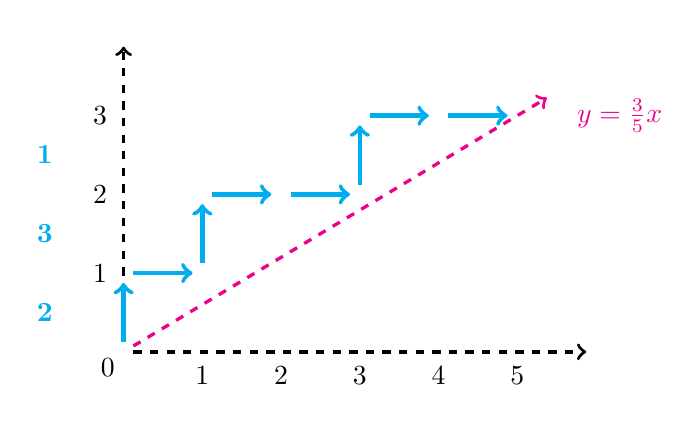
\begin{tikzpicture}[scale=1]
        \node (a) at (0, 0) {};
        \node (b) at (0, 4) {};
        \node (c) at (6, 0) {};
        \node (d) at (5.5, 3.3) {};
        \node (e) at (6.3, 3) [color = magenta]
            {$y = \frac{3}{5}x$}; 
        \draw [dashed, very thick, ->] (a) to (b);
        \draw [dashed, very thick, ->] (a) to (c);
        \draw [dashed, very thick, ->]
            [color = magenta] (a) to (d);

        \node (1)  at (0,0)   {};
        \node (2)  at (0,1)   {};
        \node (3)  at (1,1)   {};
        \node (4)  at (1,2)   {};
        \node (5)  at (2,2)   {};
        \node (6)  at (3,2)   {};
        \node (7)  at (3,3)   {};
        \node (8)  at (4,3)   {};
        \node (9)  at (5,3)   {};
        \draw [->, ultra thick, color = cyan]
            (1)  to (2);
        \draw [->, ultra thick, color = cyan] 
            (2)  to (3);
        \draw [->, ultra thick, color = cyan]
            (3)  to (4);
        \draw [->, ultra thick, color = cyan]
            (4)  to (5);
        \draw [->, ultra thick, color = cyan]
            (5)  to (6);
        \draw [->, ultra thick, color = cyan]
            (6)  to (7);
        \draw [->, ultra thick, color = cyan]
            (7)  to (8);
        \draw [->, ultra thick, color = cyan]
            (8)  to (9);

        \node at (-0.2, -0.2) {$0$};
        \node at (-0.3, 1)    {$1$};
        \node at (1, -0.3)    {$1$};
        \node at (-0.3, 2)    {$2$};
        \node at (2, -0.3)    {$2$};
        \node at (-0.3, 3)    {$3$};
        \node at (3, -0.3)    {$3$};
        \node at (4, -0.3)    {$4$};
        \node at (5, -0.3)    {$5$};

        \node [color = cyan] at (-1, 0.5) {\textbf{2}};
        \node [color = cyan] at (-1, 1.5) {\textbf{3}};
        \node [color = cyan] at (-1, 2.5) {\textbf{1}};

    \end{tikzpicture}
\end{center}
\end{example}

\begin{example}[$a > b : a = 7, b = 3,
        \mathcal{LR}_{a,b} \to \mathcal{PF}_{a,b}$]
    ~\
    \begin{itemize}
        \item $w = 2570134060$
    \end{itemize}
    \begin{center}
        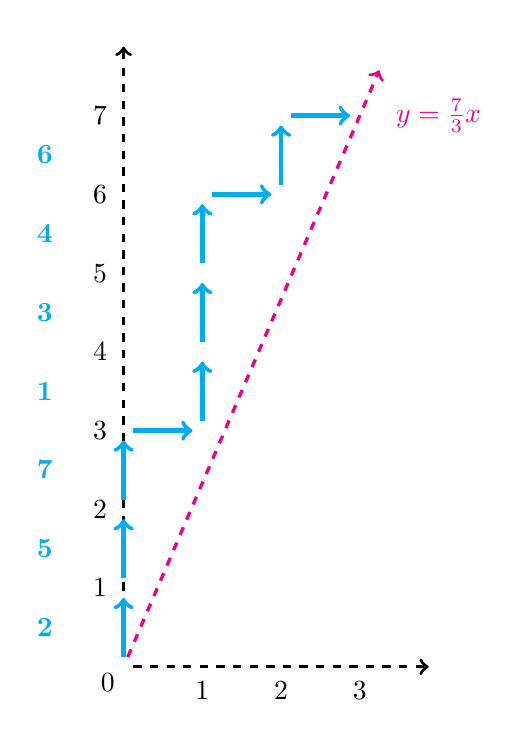
\begin{tikzpicture}[scale=1]
            \node (a) at (0, 0) {};
            \node (b) at (0, 8) {};
            \node (c) at (4, 0) {};
            \node (d) at (3.3, 7.7) {};
            \node (e) at (4, 7) [color = magenta]
                {$y = \frac{7}{3}x$}; 
            \draw [dashed, very thick, ->] (a) to (b);
            \draw [dashed, very thick, ->] (a) to (c);
            \draw [dashed, very thick, ->]
                [color = magenta] (a) to (d);

            \node (1)  at (0,0)   {};
            \node (2)  at (0,1)   {};
            \node (3)  at (0,2)   {};
            \node (4)  at (0,3)   {};
            \node (5)  at (1,3)   {};
            \node (6)  at (1,4)   {};
            \node (7)  at (1,5)   {};
            \node (8)  at (1,6)   {};
            \node (9)  at (2,6)   {};
            \node (10) at (2,7)   {};
            \node (11) at (3,7)   {};
            \draw [->, ultra thick, color = cyan]
                (1)  to (2);
            \draw [->, ultra thick, color = cyan] 
                (2)  to (3);
            \draw [->, ultra thick, color = cyan]
                (3)  to (4);
            \draw [->, ultra thick, color = cyan]
                (4)  to (5);
            \draw [->, ultra thick, color = cyan]
                (5)  to (6);
            \draw [->, ultra thick, color = cyan]
                (6)  to (7);
            \draw [->, ultra thick, color = cyan]
                (7)  to (8);
            \draw [->, ultra thick, color = cyan]
                (8)  to (9);
            \draw [->, ultra thick, color = cyan]
                (9)  to (10);
            \draw [->, ultra thick, color = cyan]
                (10) to (11);

            \node at (-0.2, -0.2) {$0$};
            \node at (-0.3, 1)    {$1$};
            \node at (1, -0.3)    {$1$};
            \node at (-0.3, 2)    {$2$};
            \node at (2, -0.3)    {$2$};
            \node at (-0.3, 3)    {$3$};
            \node at (3, -0.3)    {$3$};
            \node at (-0.3, 4)    {$4$};
            \node at (-0.3, 5)    {$5$};
            \node at (-0.3, 6)    {$6$};
            \node at (-0.3, 7)    {$7$};

            \node [color = cyan] at (-1, 0.5) {\textbf{2}};
            \node [color = cyan] at (-1, 1.5) {\textbf{5}};
            \node [color = cyan] at (-1, 2.5) {\textbf{7}};
            \node [color = cyan] at (-1, 3.5) {\textbf{1}};
            \node [color = cyan] at (-1, 4.5) {\textbf{3}};
            \node [color = cyan] at (-1, 5.5) {\textbf{4}};
            \node [color = cyan] at (-1, 6.5) {\textbf{6}};
        \end{tikzpicture}
    \end{center}

    \begin{itemize}
        \item Distances :
            \subitem $s_1 = 0$
            \hspace{2cm} $s_2 = 0$
            \hspace{2cm} $s_3 = 0$
            \subitem $s_4 = 1$
            \hspace{2cm} $s_5 = 1$
            \hspace{2cm} $s_6 = 1$
            \subitem $s_7 = 2$
        \item Labels :
            \subitem $dist_0 = \{2, 5, 7\}$
            \hspace{2cm} $dist_1 = \{1, 3, 4\}$
            \hspace{2cm} $dist_2 = \{6\}$
        \item $f = (2, 1, 2, 2, 1, 3, 1)$
    \end{itemize}
\end{example}

\begin{example}[$a < b : a = 3, b = 5,
    \mathcal{LR}_{a,b} \to \mathcal{PF}_{a,b}$]
~\
\begin{itemize}
    \item $w = 13000200$
\end{itemize}
\begin{center}
    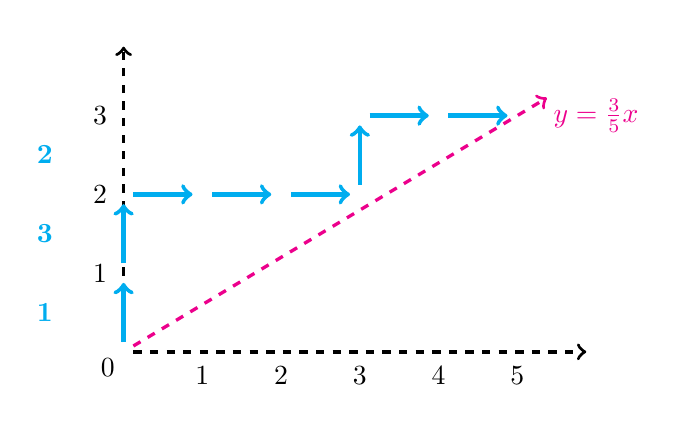
\begin{tikzpicture}[scale=1]
        \node (a) at (0, 0) {};
        \node (b) at (0, 4) {};
        \node (c) at (6, 0) {};
        \node (d) at (5.5, 3.3) {};
        \node (e) at (6, 3) [color = magenta]
            {$y = \frac{3}{5}x$}; 
        \draw [dashed, very thick, ->] (a) to (b);
        \draw [dashed, very thick, ->] (a) to (c);
        \draw [dashed, very thick, ->]
            [color = magenta] (a) to (d);

        \node (1)  at (0,0)   {};
        \node (2)  at (0,1)   {};
        \node (3)  at (0,2)   {};
        \node (4)  at (1,2)   {};
        \node (5)  at (2,2)   {};
        \node (6)  at (3,2)   {};
        \node (7)  at (3,3)   {};
        \node (8)  at (4,3)   {};
        \node (9)  at (5,3)   {};
        \draw [->, ultra thick, color = cyan]
            (1)  to (2);
        \draw [->, ultra thick, color = cyan] 
            (2)  to (3);
        \draw [->, ultra thick, color = cyan]
            (3)  to (4);
        \draw [->, ultra thick, color = cyan]
            (4)  to (5);
        \draw [->, ultra thick, color = cyan]
            (5)  to (6);
        \draw [->, ultra thick, color = cyan]
            (6)  to (7);
        \draw [->, ultra thick, color = cyan]
            (7)  to (8);
        \draw [->, ultra thick, color = cyan]
            (8)  to (9);

        \node at (-0.2, -0.2) {$0$};
        \node at (-0.3, 1)    {$1$};
        \node at (1, -0.3)    {$1$};
        \node at (-0.3, 2)    {$2$};
        \node at (2, -0.3)    {$2$};
        \node at (-0.3, 3)    {$3$};
        \node at (3, -0.3)    {$3$};
        \node at (4, -0.3)    {$4$};
        \node at (5, -0.3)    {$5$};

        \node [color = cyan] at (-1, 0.5) {\textbf{1}};
        \node [color = cyan] at (-1, 1.5) {\textbf{3}};
        \node [color = cyan] at (-1, 2.5) {\textbf{2}};
    \end{tikzpicture}
\end{center}

\begin{itemize}
    \item Distances :
        \subitem $s_1 = 0$
        \hspace{2cm} $s_2 = 0$
        \hspace{2cm} $s_3 = 3$
    \item Labels :
        \subitem $dist_0 = \{1, 3\}$
        \hspace{2cm} $dist_1 = \emptyset$
        \hspace{2cm} $dist_2 = \emptyset$
        \subitem $dist_3 = \{2\}$
        \hspace{2cm} $dist_4 = \emptyset$
    \item $f = (1, 4, 1)$
\end{itemize}
\end{example}

\begin{rem}
    The rational primitive parking functions are exactly the
    rational parking functions corresponding to rational labeled
    Dyck paths where the $i^{th}$ North step is labeled $i$.
\end{rem}

\subsection{Rational Dyck - Parking Posets}

\subsubsection{Rational Primitive Dyck - Parking Posets}

\begin{definition}[$\gtrdot_r$]
    For $w$ and $w'$ two a, b - Dyck words, we say that $w$
    covers $w'$, written $w \gtrdot_r w'$, if
    $\exists w_1, w_2$ such that :
    \begin{itemize}
        \item $w = w_101w_2$
        \item $w' = w_110w_2$
    \end{itemize}  
\end{definition}

\begin{example}[$a = 7, b = 3$]
    $1111011010 \gtrdot_r 1111011100$
    \begin{itemize}
        \item $w_1 = 1111011$
        \item $w_2 = 0$
    \end{itemize}
    \begin{center}
        \begin{tikzpicture}[scale=1]
            \node (a) at (0, 0) {};
            \node (b) at (0, 8) {};
            \node (c) at (4, 0) {};
            \node (d) at (3.3, 7.7) {};
            \node (e) at (4, 7) [color = magenta]
                {$y = \frac{7}{3}x$}; 
            \draw [dashed, very thick, ->] (a) to (b);
            \draw [dashed, very thick, ->] (a) to (c);
            \draw [dashed, very thick, ->]
                [color = magenta] (a) to (d);

            \node (1)  at (0,0)   {};
            \node (2)  at (0,1)   {};
            \node (3)  at (0,2)   {};
            \node (4)  at (0,3)   {};
            \node (5)  at (0,4)   {};
            \node (6)  at (1,4)   {};
            \node (7)  at (1,5)   {};
            \node (8)  at (1,6)   {};
            \node (9)  at (2,6)   {};
            \node (9b) at (1,7)   {};
            \node (10) at (2,7)   {};
            \node (11) at (3,7)   {};

            \draw [->, ultra thick, color = cyan]
                (1)  to (2);
            \draw [->, ultra thick, color = cyan] 
                (2)  to (3);
            \draw [->, ultra thick, color = cyan]
                (3)  to (4);
            \draw [->, ultra thick, color = cyan]
                (4)  to (5);
            \draw [->, ultra thick, color = cyan]
                (5)  to (6);
            \draw [->, ultra thick, color = cyan]
                (6)  to (7);
            \draw [->, ultra thick, color = cyan]
                (7)  to (8);
            \draw [->, ultra thick, color = cyan]
                (8)  to (9);
            \draw [->, ultra thick, color = cyan]
                (9)  to (10);
            \draw [->, ultra thick, color = cyan]
                (10) to (11);

            \draw [->, dashed, ultra thick, color = violet]
                (1)  to (2);
            \draw [->, dashed, ultra thick, color = violet] 
                (2)  to (3);
            \draw [->, dashed, ultra thick, color = violet]
                (3)  to (4);
            \draw [->, dashed, ultra thick, color = violet]
                (4)  to (5);
            \draw [->, dashed, ultra thick, color = violet]
                (5)  to (6);
            \draw [->, dashed, ultra thick, color = violet]
                (6)  to (7);
            \draw [->, dashed, ultra thick, color = violet]
                (7)  to (8);
            \draw [->, ultra thick, color = violet]
                (8)  to (9b);
            \draw [->, ultra thick, color = violet]
                (9b)  to (10);
            \draw [->, dashed, ultra thick, color = violet]
                (10) to (11);

            \node at (-0.2, -0.2) {$0$};
            \node at (-0.3, 1)    {$1$};
            \node at (1, -0.3)    {$1$};
            \node at (-0.3, 2)    {$2$};
            \node at (2, -0.3)    {$2$};
            \node at (-0.3, 3)    {$3$};
            \node at (3, -0.3)    {$3$};
            \node at (-0.3, 4)    {$4$};
            \node at (-0.3, 5)    {$5$};
            \node at (-0.3, 6)    {$6$};
            \node at (-0.3, 7)    {$7$};

            \draw[color = red, ultra thick]
                (1.1,6.1) -- (1.9,6.9);
            \draw[color = red, ultra thick]
                (1.1,6.4) -- (1.6,6.9);
            \draw[color = red, ultra thick]
                (1.15,6.7) -- (1.35,6.9);
            \draw[color = red, ultra thick]
                (1.4,6.1) -- (1.9,6.6);
            \draw[color = red, ultra thick]
                (1.7,6.15) -- (1.9,6.35);

            \fill[color = cyan] (-2.7,-1.9) rectangle
                (-2.2,-1.7);
            \node at (-0.7,-1.8) {$1111011010$};
            \fill[color = violet] (2,-1.9) rectangle
            (2.5,-1.7);
            \node at (4,-1.8) {$1111011100$};
            \fill[color = red] (6.7,-1.9) rectangle
            (7.2,-1.7);
            \node at (8.5,-1.8) {difference};
        \end{tikzpicture}
    \end{center}
\end{example}

\begin{rem}
    If $w_1 \gtrdot_r w_2$, then the path corresponding to
    $w_2$ is \emph{over} the path corresponding to $w_1$,
    and the \emph{difference} between the two paths is a
    square of size 1 by 1.
\end{rem}

\begin{prop}
    This covering relation defines a \emph{poset}
    for $\mathcal{R}_{a,b}$.
\end{prop}

\begin{example}[$a > b$ : The poset of $\mathcal{R}_{5,3}$]
    ~\\
    \begin{center}
        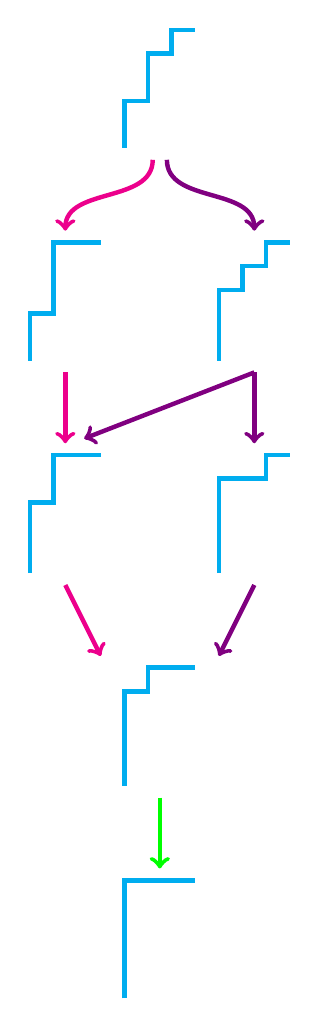
\begin{tikzpicture}[scale = 0.3]
            \draw [ultra thick, color = cyan] (0,0) -- (0,1)
                -- (0,2) -- (0,3) -- (0,4) -- (0,5) -- (1,5)
                -- (2,5) -- (3,5);

            \draw [ultra thick, color = cyan] (0,9) -- (0,10)
                -- (0,11) -- (0,12) -- (0,13) -- (1,13) -- (1,14)
                -- (2,14) -- (3,14);
                
            \draw [ultra thick, color = cyan] (-4,18) -- (-4,19)
                -- (-4,20) -- (-4,21) -- (-3,21) -- (-3,22)
                -- (-3,23) -- (-2,23) -- (-1,23);

            \draw [ultra thick, color = cyan] (4,18) -- (4,19)
                -- (4,20) -- (4,21) -- (4,22) -- (5,22) -- (6,22)
                -- (6,23) -- (7,23);

            \draw [ultra thick, color = cyan] (-4,27) -- (-4,28)
                -- (-4,29) -- (-3,29) -- (-3,30) -- (-3,31)
                -- (-3,32) -- (-2,32) -- (-1,32);

            \draw [ultra thick, color = cyan] (4,27) -- (4,28)
                -- (4,29) -- (4,30) -- (5,30) -- (5,31) -- (6,31)
                -- (6,32) -- (7,32);

            \draw [ultra thick, color = cyan] (0,36) -- (0,37)
                -- (0,38) -- (1,38) -- (1,39) -- (1,40) -- (2,40)
                -- (2,41) -- (3,41);

            \draw [->][out=-90,in=90, ultra thick] 
                [color=magenta](1.2,35.5) to (-2.5,32.5);
            \draw [->][color=magenta, ultra thick]
                (-2.5,26.5) to (-2.5,23.5);
            \draw [->][color=magenta, ultra thick]
                (-2.5,17.5) to (-1,14.5);        

            \draw [->][out=-90,in=90, ultra thick] 
                [color=green](1.5,8.5) to (1.5,5.5);
        
            \draw [->][out=-90,in=90, ultra thick]
                [color=violet](1.8,35.5) to (5.5,32.5);
            \draw [->][color=violet, ultra thick]
                (5.5,26.5) to (5.5,23.5);
            \draw [->][color=violet, ultra thick]
                (5.5,26.5) to (-1.7,23.7);
            \draw [->][color=violet, ultra thick]
                (5.5,17.5) to (4,14.5);
        
        \end{tikzpicture}
        ~\\
        ~\\
        There are $\frac {1}{8} \binom{8}{5} = \frac{42}{6} = 7$
        elements in this poset.
    \end{center}
\end{example}

\begin{example}[$a < b$ : The poset of $\mathcal{R}_{3,7}$]
    ~\\
    \begin{center}
        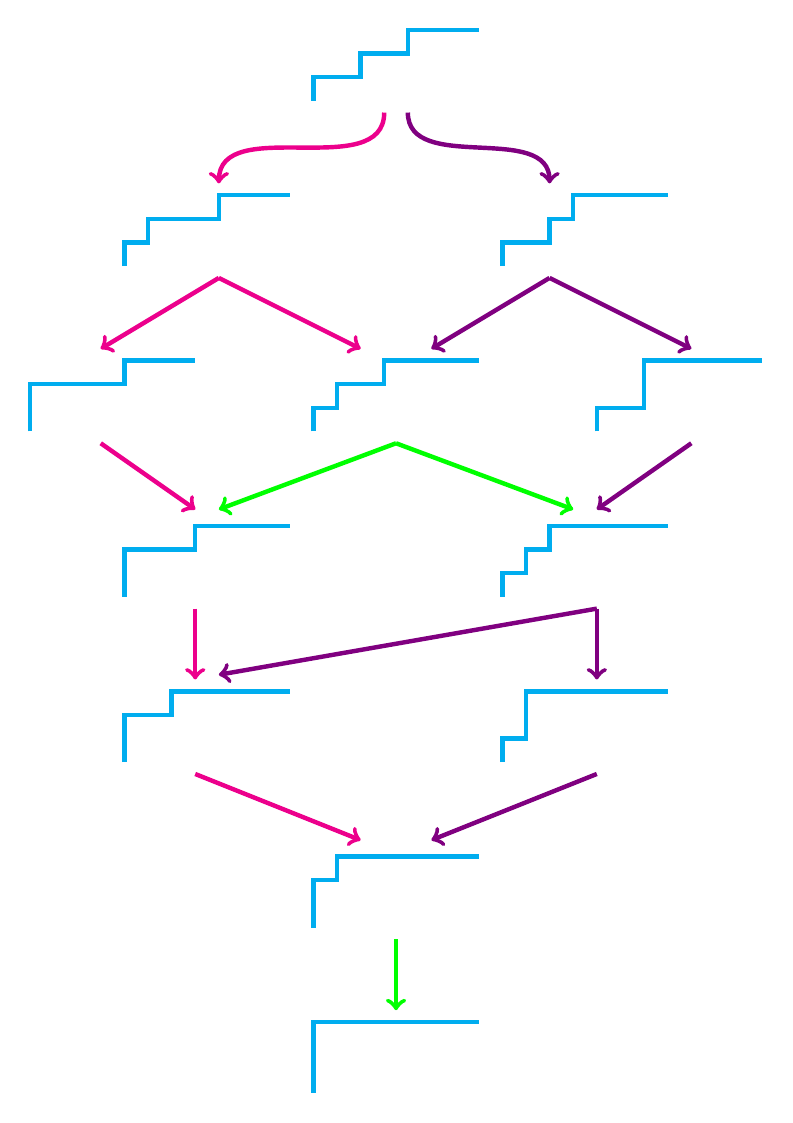
\begin{tikzpicture}[scale = 0.3]
            \draw [ultra thick, color = cyan] (0,0) -- (0,1)
                -- (0,2) -- (0,3) -- (1,3) -- (2,3) -- (3,3)
                -- (4,3) -- (5,3) -- (6,3) -- (7,3);

            \draw [ultra thick, color = cyan] (0,7) -- (0,8)
                -- (0,9) -- (1,9) -- (1,10) -- (2,10) -- (3,10)
                -- (4,10) -- (5,10) -- (6,10) -- (7,10);

            \draw [ultra thick, color = cyan] (-8,14) -- (-8,15)
                -- (-8,16) -- (-7,16) -- (-6,16) -- (-6,17) -- (-5,17)
                -- (-4,17) -- (-3,17) -- (-2,17) -- (-1,17);
                
            \draw [ultra thick, color = cyan] (8,14) -- (8,15)
                -- (9,15) -- (9,16) -- (9,17) -- (10,17)
                -- (11,17) -- (12,17) -- (13,17) -- (14,17)
                -- (15,17);

            \draw [ultra thick, color = cyan] (-8,21) -- (-8,22)
                -- (-8,23) -- (-7,23) -- (-6,23) -- (-5,23)
                -- (-5,24) -- (-4,24) -- (-3,24) -- (-2,24)
                -- (-1, 24);

            \draw [ultra thick, color = cyan] (8,21) -- (8,22)
                -- (9,22) -- (9,23) -- (10,23) -- (10,24) -- (11,24)
                -- (12,24) -- (13,24) -- (14,24) -- (15,24);
    
            \draw [ultra thick, color = cyan] (-12,28) -- (-12,29)
                -- (-12,30) -- (-11,30) -- (-10,30) -- (-9,30) -- (-8,30)
                -- (-8,31) -- (-7,31) -- (-6,31) -- (-5,31);

            \draw [ultra thick, color = cyan] (0,28) -- (0,29)
                -- (1,29) -- (1,30) -- (2,30) -- (3,30) -- (3,31)
                -- (4,31) -- (5,31) -- (6,31) -- (7,31);

            \draw [ultra thick, color = cyan] (12,28) -- (12,29)
                -- (13,29) -- (14,29) -- (14,30) -- (14,31) -- (15,31)
                -- (16,31) -- (17,31) -- (18,31) -- (19,31);

            \draw [ultra thick, color = cyan] (-8,35) -- (-8,36)
                -- (-7,36) -- (-7,37) -- (-6,37) -- (-5,37) -- (-4,37)
                -- (-4,38) -- (-3,38) -- (-2,38) -- (-1,38);

            \draw [ultra thick, color = cyan] (8,35) -- (8,36)
                -- (9,36) -- (10,36) -- (10,37) -- (11,37) -- (11,38)
                -- (12,38) -- (13,38) -- (14,38) -- (15,38);

            \draw [ultra thick, color = cyan] (0,42) -- (0,43)
                -- (1,43) -- (2,43) -- (2,44) -- (3,44) -- (4,44)
                -- (4,45) -- (5,45) -- (6,45) -- (7,45);

            \draw [->][out=-90,in=90, ultra thick] 
                [color=magenta](3,41.5) to (-4,38.5);
            \draw [->][color=magenta, ultra thick]
                (-4,34.5) to (-9,31.5);
            \draw [->][color=magenta, ultra thick]
                (-4,34.5) to (2,31.5);        
            \draw [->][color=magenta, ultra thick]
                (-9,27.5) to (-5,24.7);
            \draw [->][color=magenta, ultra thick]
                (-5,20.5) to (-5,17.5);
            \draw [->][color=magenta, ultra thick]
                (-5,13.5) to (2,10.7);

            \draw [->][color=green, ultra thick]
                (3.5,27.5) to (-4,24.7);
            \draw [->][color=green, ultra thick]
                (3.5,27.5) to (11,24.7);
            \draw [->][out=-90,in=90, ultra thick] 
                [color=green](3.5,6.5) to (3.5,3.5);
        
            \draw [->][out=-90,in=90, ultra thick]
                [color=violet](4,41.5) to (10,38.5);
            \draw [->][color=violet, ultra thick]
                (10,34.5) to (5,31.5);
            \draw [->][color=violet, ultra thick]
                (10,34.5) to (16,31.5);
            \draw [->][color=violet, ultra thick]
                (16,27.5) to (12,24.7);
            \draw [->][color=violet, ultra thick]
                (12,20.5) to (-4,17.7);
            \draw [->][color=violet, ultra thick]
                (12,20.5) to (12,17.5);
            \draw [->][color=violet, ultra thick]
                (12,13.5) to (5,10.7);
        
        \end{tikzpicture}
        ~\\
        ~\\
        There are $\frac {1}{10} \binom{10}{3} = \frac{72}{6} = 12$
        elements in this poset.
    \end{center}
\end{example}

\begin{definition}[$\gtrdot'$]
    For $f$ and $g$ two rational primitive a, b - parking 
    functions, we say that $f$ covers $g$, written
    $f \gtrdot' g$, if $\exists i$ such that :
    \begin{itemize}
        \item $f = (a_1, \ldots, a_{i-1}, a_i,\ \ \ \ 
            a_{i+1}, \ldots, a_n)$
        \item $g = (a_1, \ldots, a_{i-1}, a_i - 1, a_{i+1},
        \ldots, a_n)$
    \end{itemize}
\end{definition}

\begin{example}[$a > b : a = 7, b = 3$]
    $(1, 1, 1, 2, 2, 2, 3) \gtrdot' (1, 1, 1, 1, 2, 2, 3)$    
\end{example}

\begin{example}[$a < b : a = 3, b = 5$]
    $(1, 2, 4) \gtrdot' (1, 1, 4)$    
\end{example}

\begin{prop}
    This covering relation defines a \emph{poset}
    for $\mathcal{PF'}_{a,b}$.
\end{prop}

\begin{example}[$a > b$ : The poset of $\mathcal{PF'}_{5,3}$]
    ~\\
    \begin{center}
        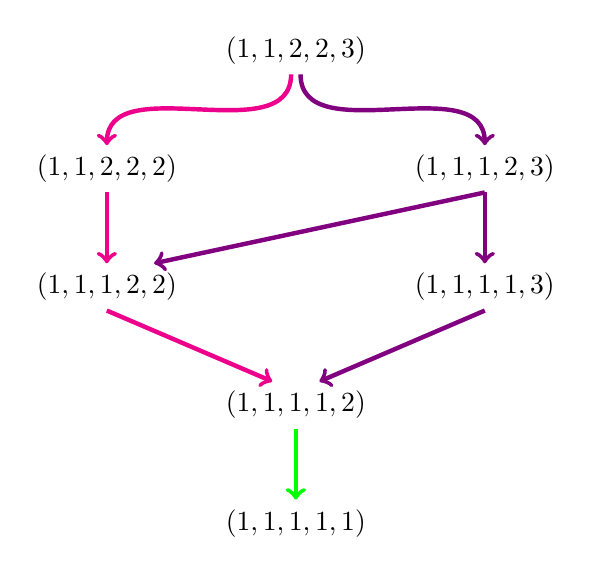
\begin{tikzpicture}[scale = 0.3]
            \node at (0,0) {$(1, 1, 1, 1, 1)$};

            \node at (0,5) {$(1, 1, 1, 1, 2)$};
                
            \node at (-8,10) {$(1, 1, 1, 2, 2)$};
            \node at (8,10)  {$(1, 1, 1, 1, 3)$};

            \node at (-8,15) {$(1, 1, 2, 2, 2)$};
            \node at (8,15)  {$(1, 1, 1, 2, 3)$};

            \node at (0,20) {$(1, 1, 2, 2, 3)$};

            \draw [->][out=-90,in=90, ultra thick] 
                [color=magenta](-0.2,19) to (-8,16);
            \draw [->][color=magenta, ultra thick]
                (-8,14) to (-8,11);
            \draw [->][color=magenta, ultra thick]
                (-8,9) to (-1,6);        

            \draw [->][out=-90,in=90, ultra thick] 
                [color=green](0,4) to (0,1);
        
            \draw [->][out=-90,in=90, ultra thick]
                [color=violet](0.2,19) to (8,16);
            \draw [->][color=violet, ultra thick]
                (8,14) to (-6,11);
            \draw [->][color=violet, ultra thick]
                (8,14) to (8,11);
            \draw [->][color=violet, ultra thick]
                (8,9) to (1,6);
        
        \end{tikzpicture}
        ~\\
        ~\\
        There are $\frac {1}{8} \binom{8}{5} = \frac{42}{6} = 7$
        elements in this poset.
    \end{center}
\end{example}

\begin{example}[$a < b$ : The poset of $\mathcal{PF'}_{3,7}$]
    ~\\
    \begin{center}
        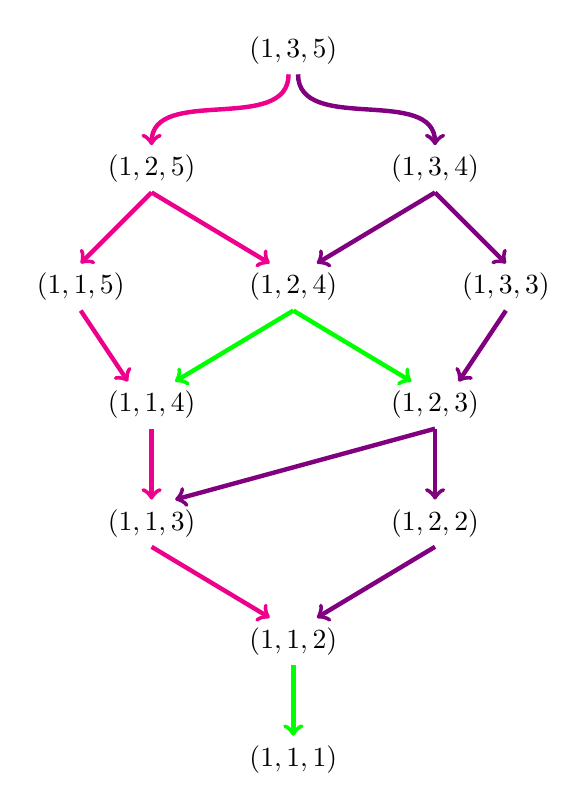
\begin{tikzpicture}[scale = 0.3]
            \node at (0,0) {$(1,1,1)$};

            \node at (0,5) {$(1,1,2)$};

            \node at (-6,10) {$(1,1,3)$};                
            \node at (6,10)  {$(1,2,2)$};

            \node at (-6,15) {$(1,1,4)$};
            \node at (6,15)  {$(1,2,3)$};
    
            \node at (-9,20) {$(1,1,5)$};
            \node at (0,20)  {$(1,2,4)$};
            \node at (9,20)  {$(1,3,3)$};

            \node at (-6,25) {$(1,2,5)$};
            \node at (6,25)  {$(1,3,4)$};

            \node at (0,30) {$(1,3,5)$};

            \draw [->][out=-90,in=90, ultra thick] 
                [color=magenta](-0.2,29) to (-6,26);
            \draw [->][color=magenta, ultra thick]
                (-6,24) to (-9,21);
            \draw [->][color=magenta, ultra thick]
                (-6,24) to (-1,21);        
            \draw [->][color=magenta, ultra thick]
                (-9,19) to (-7,16);
            \draw [->][color=magenta, ultra thick]
                (-6,14) to (-6,11);
            \draw [->][color=magenta, ultra thick]
                (-6,9) to (-1,6);

            \draw [->][color=green, ultra thick]
                (0,19) to (-5,16);
            \draw [->][color=green, ultra thick]
                (0,19) to (5,16);
            \draw [->][out=-90,in=90, ultra thick] 
                [color=green](0,4) to (0,1);
        
            \draw [->][out=-90,in=90, ultra thick]
                [color=violet](0.2,29) to (6,26);
            \draw [->][color=violet, ultra thick]
                (6,24) to (1,21);
            \draw [->][color=violet, ultra thick]
                (6,24) to (9,21);
            \draw [->][color=violet, ultra thick]
                (9,19) to (7,16);
            \draw [->][color=violet, ultra thick]
                (6,14) to (-5,11);
            \draw [->][color=violet, ultra thick]
                (6,14) to (6,11);
            \draw [->][color=violet, ultra thick]
                (6,9) to (1,6);
        
        \end{tikzpicture}
        ~\\
        ~\\
        There are $\frac {1}{10} \binom{10}{3} = \frac{72}{6} = 12$
        elements in this poset.
    \end{center}
\end{example}

\begin{rem}
    The posets of $\mathcal{PF'}_{a,b}$ and $\mathcal{R}_{a,b}$
    are isomorphic, and one can be obtained by
    applying the aforementioned bijection to the other.
\end{rem}

\subsubsection{Rational Dyck - Parking Posets}

\begin{definition}[$\gtrdot_{lr}$]
    For $w$ and $w'$ two labeled a, b - Dyck words, we say
    that $w$ covers $w'$, written $w \gtrdot_{lr} w'$,
    if either :
    \begin{itemize}
        \item $\exists w_2, x, x', y$ such that :
            \subitem $x = x_1x_2 \cdots x_n$ has all 
            its digits $> 0$
            \subitem $x' = x$ where $y$ is correctly
            inserted regarding the order condition
            \subitem $y > 0$
            \subitem $w = x0yw_2$
            \subitem $w' = x'0w_2$
        \item $\exists w_1, w_2, x, x', y$ such that :
            \subitem $x = x_1x_2 \cdots x_n$ has all 
                its digits $> 0$
            \subitem $y > 0$
            \subitem $x' = x$ where $y$ is correctly
                inserted regarding the order condition
            \subitem $w = w_10x0yw_2$
            \subitem $w' = w_10x'0w_2$
        \item or $\exists w_1, w_2, y$ such that :
            \subitem $y > 0$
            \subitem $w = w_100yw_2$
            \subitem $w' = w_10y0w_2$
    \end{itemize}  
\end{definition}

\begin{example}[$a > b : a = 7, b = 3$, first case]
    $1457030260 \gtrdot_{lr} 1345700260$
    \begin{itemize}
        \item $w_2 = 0260$
        \item $x = 1457$
        \item $x' = 13457$
        \item $y = 3$
    \end{itemize}

    \begin{center}
        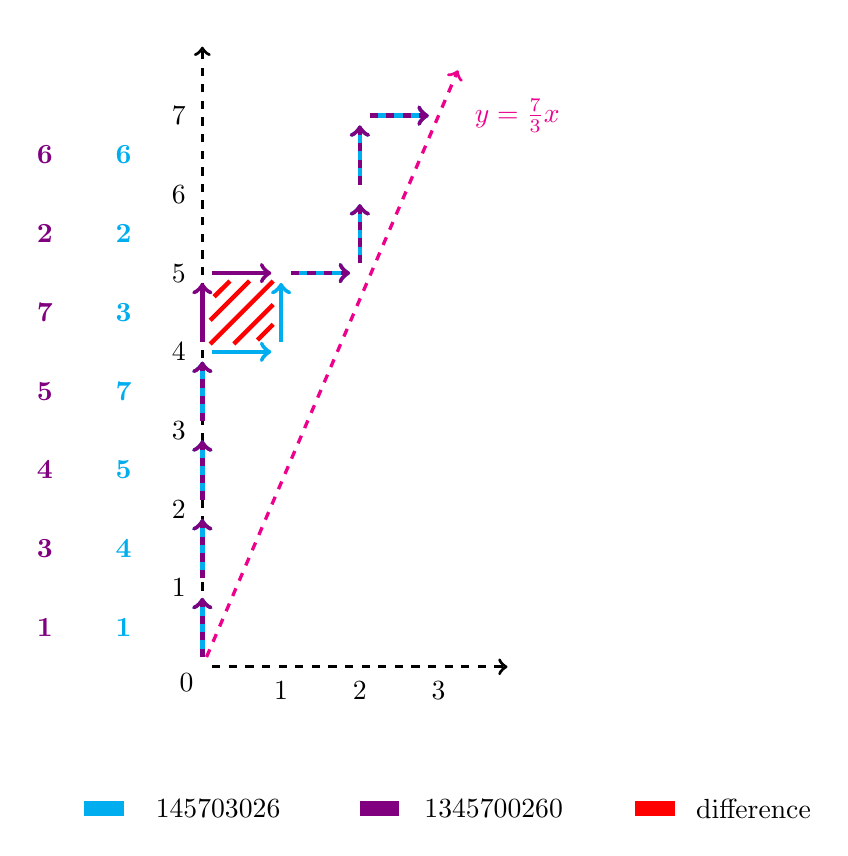
\begin{tikzpicture}[scale=1]
            \node (a) at (0, 0) {};
            \node (b) at (0, 8) {};
            \node (c) at (4, 0) {};
            \node (d) at (3.3, 7.7) {};
            \node (e) at (4, 7) [color = magenta]
                {$y = \frac{7}{3}x$}; 
            \draw [dashed, very thick, ->] (a) to (b);
            \draw [dashed, very thick, ->] (a) to (c);
            \draw [dashed, very thick, ->]
                [color = magenta] (a) to (d);

            \node (1)  at (0,0)   {};
            \node (2)  at (0,1)   {};
            \node (3)  at (0,2)   {};
            \node (4)  at (0,3)   {};
            \node (5)  at (0,4)   {};
            \node (6)  at (1,4)   {};
            \node (6b) at (0,5)   {};
            \node (7)  at (1,5)   {};
            \node (8)  at (2,5)   {};
            \node (9)  at (2,6)   {};
            \node (10) at (2,7)   {};
            \node (11) at (3,7)   {};

            \draw [->, ultra thick, color = cyan]
                (1)  to (2);
            \draw [->, ultra thick, color = cyan] 
                (2)  to (3);
            \draw [->, ultra thick, color = cyan]
                (3)  to (4);
            \draw [->, ultra thick, color = cyan]
                (4)  to (5);
            \draw [->, ultra thick, color = cyan]
                (5)  to (6);
            \draw [->, ultra thick, color = cyan]
                (6)  to (7);
            \draw [->, ultra thick, color = cyan]
                (7)  to (8);
            \draw [->, ultra thick, color = cyan]
                (8)  to (9);
            \draw [->, ultra thick, color = cyan]
                (9)  to (10);
            \draw [->, ultra thick, color = cyan]
                (10) to (11);

            \draw [->, dashed, ultra thick, color = violet]
                (1)  to (2);
            \draw [->, dashed, ultra thick, color = violet] 
                (2)  to (3);
            \draw [->, dashed, ultra thick, color = violet]
                (3)  to (4);
            \draw [->, dashed, ultra thick, color = violet]
                (4)  to (5);
            \draw [->, ultra thick, color = violet]
                (5)  to (6b);
            \draw [->, ultra thick, color = violet]
                (6b)  to (7);
            \draw [->, dashed, ultra thick, color = violet]
                (7)  to (8);
            \draw [->, dashed, ultra thick, color = violet]
                (8)  to (9);
            \draw [->, dashed, ultra thick, color = violet]
                (9)  to (10);
            \draw [->, dashed, ultra thick, color = violet]
                (10) to (11);

            \node at (-0.2, -0.2) {$0$};
            \node at (-0.3, 1)    {$1$};
            \node at (1, -0.3)    {$1$};
            \node at (-0.3, 2)    {$2$};
            \node at (2, -0.3)    {$2$};
            \node at (-0.3, 3)    {$3$};
            \node at (3, -0.3)    {$3$};
            \node at (-0.3, 4)    {$4$};
            \node at (-0.3, 5)    {$5$};
            \node at (-0.3, 6)    {$6$};
            \node at (-0.3, 7)    {$7$};

            \node [color = cyan] at (-1, 0.5) {\textbf{1}};
            \node [color = cyan] at (-1, 1.5) {\textbf{4}};
            \node [color = cyan] at (-1, 2.5) {\textbf{5}};
            \node [color = cyan] at (-1, 3.5) {\textbf{7}};
            \node [color = cyan] at (-1, 4.5) {\textbf{3}};
            \node [color = cyan] at (-1, 5.5) {\textbf{2}};
            \node [color = cyan] at (-1, 6.5) {\textbf{6}};


            \node [color = violet] at (-2, 0.5) {\textbf{1}};
            \node [color = violet] at (-2, 1.5) {\textbf{3}};
            \node [color = violet] at (-2, 2.5) {\textbf{4}};
            \node [color = violet] at (-2, 3.5) {\textbf{5}};
            \node [color = violet] at (-2, 4.5) {\textbf{7}};
            \node [color = violet] at (-2, 5.5) {\textbf{2}};
            \node [color = violet] at (-2, 6.5) {\textbf{6}};

            \draw[color = red, ultra thick]
                (0.1,4.1) -- (0.9,4.9);
            \draw[color = red, ultra thick]
                (0.1,4.4) -- (0.6,4.9);
            \draw[color = red, ultra thick]
                (0.15,4.7) -- (0.35,4.9);
            \draw[color = red, ultra thick]
                (0.4,4.1) -- (0.9,4.6);
            \draw[color = red, ultra thick]
                (0.7,4.15) -- (0.9,4.35);

            \fill[color = cyan] (-1,-1.9) rectangle
                (-1.5,-1.7);0
            \node at (0.2,-1.8) {$145703026$};
            \fill[color = violet] (2,-1.9) rectangle
                (2.5,-1.7);
            \node at (3.7,-1.8) {$1345700260$};
            \fill[color = red] (6,-1.9) rectangle
                (5.5,-1.7);
            \node at (7,-1.8) {difference};
        \end{tikzpicture}
    \end{center}
\end{example}

\begin{example}[$a < b : a = 3, b = 5$, first case]
    $20130000 \gtrdot_{lr} 12030000$
    \begin{itemize}
        \item $w_2 = 30000$
        \item $x = 2$
        \item $x' = 12$
        \item $y = 1$
    \end{itemize}
\end{example}

\begin{example}[$a > b : a = 7, b = 3$, second case]
    $2460150370 \gtrdot_{lr} 2460135070$
    \begin{itemize}
        \item $w_1 = 246$
        \item $w_2 = 70$
        \item $x = 15$
        \item $x' = 135$
        \item $y = 3$
    \end{itemize}
\end{example}

\begin{example}[$a < b : a = 3, b = 5$, second case]
    $20301000 \gtrdot_{lr} 20130000 $
    \begin{itemize}
        \item $w_1 = 2$
        \item $w_2 = 000$
        \item $x = 3$
        \item $x' = 13$
        \item $y = 1$
    \end{itemize}
\end{example}

\begin{example}[$a > b : a = 7, b = 3$, third case]
    $235670014 \gtrdot_{lr} 235670104$
    \begin{itemize}
        \item $w_1 = 23567$
        \item $w_2 = 4$
        \item $y = 1$
    \end{itemize}
\end{example}

\begin{example}[$a < b : a = 3, b = 5$, third case]
    $23000100 \gtrdot_{lr} 23001000$
    \begin{itemize}
        \item $w_1 = 230$
        \item $w_2 = 00$
        \item $y = 1$
    \end{itemize}
\end{example}

\begin{rem}
    If $w_1 \gtrdot_{lr} w_2$, then the path corresponding to
    $w_2$ is \emph{over} the path corresponding to $w_1$,
    and the \emph{difference} between the two paths is a
    square of size 1 by 1.\\
    Furthermore, the labeling can be seen as follows :
    if one has to merge two sequences of North steps of $w_1$
    to make $w_2$, then the merging will be made by ordering the
    corresponding labels.
\end{rem}

\begin{prop}
    This covering relation defines a \emph{poset}
    for $\mathcal{LR}_{a,b}$.
\end{prop}

\begin{example}[$a > b$ : The poset of $\mathcal{LR}_{5,2}$]
    ~\\
    \begin{center}
        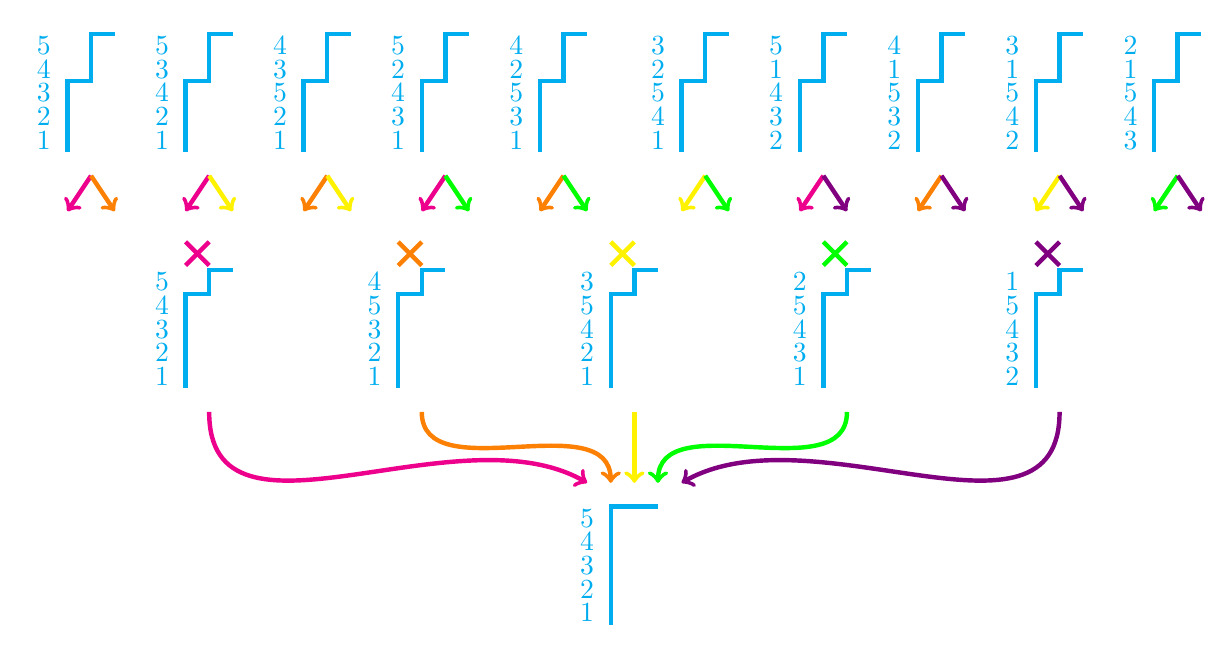
\begin{tikzpicture}[scale = 0.3]
            \draw [ultra thick, color = cyan] (0,0) -- (0,1)
                -- (0,2) -- (0,3) -- (0,4) -- (0,5) -- (1,5)
                -- (2,5);
            \node[color = cyan] at (-1,0.5) {$1$};
            \node[color = cyan] at (-1,1.5) {$2$};
            \node[color = cyan] at (-1,2.5) {$3$};
            \node[color = cyan] at (-1,3.5) {$4$};
            \node[color = cyan] at (-1,4.5) {$5$};

            \draw [ultra thick, color = cyan] (-18,10) -- (-18,11)
                -- (-18,12) -- (-18,13) -- (-18,14) -- (-17,14)
                -- (-17,15) -- (-16,15);
            \node[color = cyan] at (-19,10.5) {$1$};
            \node[color = cyan] at (-19,11.5) {$2$};
            \node[color = cyan] at (-19,12.5) {$3$};
            \node[color = cyan] at (-19,13.5) {$4$};
            \node[color = cyan] at (-19,14.5) {$5$};

            \draw [ultra thick, color = cyan] (-9,10) -- (-9,11)
                -- (-9,12) -- (-9,13) -- (-9,14) -- (-8,14)
                -- (-8,15) -- (-7,15);
            \node[color = cyan] at (-10,10.5) {$1$};
            \node[color = cyan] at (-10,11.5) {$2$};
            \node[color = cyan] at (-10,12.5) {$3$};
            \node[color = cyan] at (-10,13.5) {$5$};
            \node[color = cyan] at (-10,14.5) {$4$};

            \draw [ultra thick, color = cyan] (0,10) -- (0,11)
                -- (0,12) -- (0,13) -- (0,14) -- (1,14)
                -- (1,15) -- (2,15);
            \node[color = cyan] at (-1,10.5) {$1$};
            \node[color = cyan] at (-1,11.5) {$2$};
            \node[color = cyan] at (-1,12.5) {$4$};
            \node[color = cyan] at (-1,13.5) {$5$};
            \node[color = cyan] at (-1,14.5) {$3$};

            \draw [ultra thick, color = cyan] (9,10) -- (9,11)
                -- (9,12) -- (9,13) -- (9,14) -- (10,14)
                -- (10,15) -- (11,15);
            \node[color = cyan] at (8,10.5) {$1$};
            \node[color = cyan] at (8,11.5) {$3$};
            \node[color = cyan] at (8,12.5) {$4$};
            \node[color = cyan] at (8,13.5) {$5$};
            \node[color = cyan] at (8,14.5) {$2$};

            \draw [ultra thick, color = cyan] (18,10) -- (18,11)
                -- (18,12) -- (18,13) -- (18,14) -- (19,14)
                -- (19,15) -- (20,15);
            \node[color = cyan] at (17,10.5) {$2$};
            \node[color = cyan] at (17,11.5) {$3$};
            \node[color = cyan] at (17,12.5) {$4$};
            \node[color = cyan] at (17,13.5) {$5$};
            \node[color = cyan] at (17,14.5) {$1$};

            \draw [ultra thick, color = cyan] (-23,20) -- (-23,21)
                -- (-23,22) -- (-23,23) -- (-22,23) -- (-22,24)
                -- (-22,25) -- (-21,25);
            \node[color = cyan] at (-24,20.5) {$1$};
            \node[color = cyan] at (-24,21.5) {$2$};
            \node[color = cyan] at (-24,22.5) {$3$};
            \node[color = cyan] at (-24,23.5) {$4$};
            \node[color = cyan] at (-24,24.5) {$5$};

            \draw [ultra thick, color = cyan] (-18,20) -- (-18,21)
                -- (-18,22) -- (-18,23) -- (-17,23) -- (-17,24)
                -- (-17,25) -- (-16,25);
            \node[color = cyan] at (-19,20.5) {$1$};
            \node[color = cyan] at (-19,21.5) {$2$};
            \node[color = cyan] at (-19,22.5) {$4$};
            \node[color = cyan] at (-19,23.5) {$3$};
            \node[color = cyan] at (-19,24.5) {$5$};

            \draw [ultra thick, color = cyan] (-13,20) -- (-13,21)
                -- (-13,22) -- (-13,23) -- (-12,23) -- (-12,24)
                -- (-12,25) -- (-11,25);
            \node[color = cyan] at (-14,20.5) {$1$};
            \node[color = cyan] at (-14,21.5) {$2$};
            \node[color = cyan] at (-14,22.5) {$5$};
            \node[color = cyan] at (-14,23.5) {$3$};
            \node[color = cyan] at (-14,24.5) {$4$};

            \draw [ultra thick, color = cyan] (-8,20) -- (-8,21)
                -- (-8,22) -- (-8,23) -- (-7,23) -- (-7,24)
                -- (-7,25) -- (-6,25);
            \node[color = cyan] at (-9,20.5) {$1$};
            \node[color = cyan] at (-9,21.5) {$3$};
            \node[color = cyan] at (-9,22.5) {$4$};
            \node[color = cyan] at (-9,23.5) {$2$};
            \node[color = cyan] at (-9,24.5) {$5$};

            \draw [ultra thick, color = cyan] (-3,20) -- (-3,21)
                -- (-3,22) -- (-3,23) -- (-2,23) -- (-2,24)
                -- (-2,25) -- (-1,25);
            \node[color = cyan] at (-4,20.5) {$1$};
            \node[color = cyan] at (-4,21.5) {$3$};
            \node[color = cyan] at (-4,22.5) {$5$};
            \node[color = cyan] at (-4,23.5) {$2$};
            \node[color = cyan] at (-4,24.5) {$4$};

            \draw [ultra thick, color = cyan] (3,20) -- (3,21)
                -- (3,22) -- (3,23) -- (4,23) -- (4,24)
                -- (4,25) -- (5,25);
            \node[color = cyan] at (2,20.5) {$1$};
            \node[color = cyan] at (2,21.5) {$4$};
            \node[color = cyan] at (2,22.5) {$5$};
            \node[color = cyan] at (2,23.5) {$2$};
            \node[color = cyan] at (2,24.5) {$3$};

            \draw [ultra thick, color = cyan] (8,20) -- (8,21)
                -- (8,22) -- (8,23) -- (9,23) -- (9,24)
                -- (9,25) -- (10,25);
            \node[color = cyan] at (7,20.5) {$2$};
            \node[color = cyan] at (7,21.5) {$3$};
            \node[color = cyan] at (7,22.5) {$4$};
            \node[color = cyan] at (7,23.5) {$1$};
            \node[color = cyan] at (7,24.5) {$5$};

            \draw [ultra thick, color = cyan] (13,20) -- (13,21)
                -- (13,22) -- (13,23) -- (14,23) -- (14,24)
                -- (14,25) -- (15,25);
            \node[color = cyan] at (12,20.5) {$2$};
            \node[color = cyan] at (12,21.5) {$3$};
            \node[color = cyan] at (12,22.5) {$5$};
            \node[color = cyan] at (12,23.5) {$1$};
            \node[color = cyan] at (12,24.5) {$4$};

            \draw [ultra thick, color = cyan] (18,20) -- (18,21)
                -- (18,22) -- (18,23) -- (19,23) -- (19,24)
                -- (19,25) -- (20,25);
            \node[color = cyan] at (17,20.5) {$2$};
            \node[color = cyan] at (17,21.5) {$4$};
            \node[color = cyan] at (17,22.5) {$5$};
            \node[color = cyan] at (17,23.5) {$1$};
            \node[color = cyan] at (17,24.5) {$3$};

            \draw [ultra thick, color = cyan] (23,20) -- (23,21)
                -- (23,22) -- (23,23) -- (24,23) -- (24,24)
                -- (24,25) -- (25,25);
            \node[color = cyan] at (22,20.5) {$3$};
            \node[color = cyan] at (22,21.5) {$4$};
            \node[color = cyan] at (22,22.5) {$5$};
            \node[color = cyan] at (22,23.5) {$1$};
            \node[color = cyan] at (22,24.5) {$2$};

            \draw [->][color=magenta, ultra thick]
                (-22,19) to (-23,17.5);
            \draw [->][color=magenta, ultra thick]
                (-17,19) to (-18,17.5);
            \draw [->][color=magenta, ultra thick]
                (-7,19) to (-8,17.5);
            \draw [->][color=magenta, ultra thick]
                (9,19) to (8,17.5);
            \draw[color=magenta, ultra thick]
                (-18,16.2) -- (-17,15.2);
            \draw[color=magenta, ultra thick]
                (-18,15.2) -- (-17,16.2);
            \draw [->][out=-90,in=150, ultra thick] 
                [color=magenta](-17,9) to (-1,6);

            \draw [->][color=brown!7!orange, ultra thick]
                (-22,19) to (-21,17.5);
            \draw [->][color=brown!7!orange, ultra thick]
                (-12,19) to (-13,17.5);
            \draw [->][color=brown!7!orange, ultra thick]
                (-2,19) to (-3,17.5);
            \draw [->][color=brown!7!orange, ultra thick]
                (14,19) to (13,17.5);
            \draw[color=brown!7!orange, ultra thick]
                (-9,16.2) -- (-8,15.2);
            \draw[color=brown!7!orange, ultra thick]
                (-9,15.2) -- (-8,16.2);
            \draw [->][out=-90,in=90, ultra thick]
                [color=brown!7!orange](-8,9) to (0,6);

            \draw [->][color=yellow, ultra thick]
                (-17,19) to (-16,17.5); 
            \draw [->][color=yellow, ultra thick]
                (-12,19) to (-11,17.5); 
            \draw [->][color=yellow, ultra thick]
                (4,19) to (3,17.5); 
            \draw [->][color=yellow, ultra thick]
                (19,19) to (18,17.5); 
            \draw[color=yellow, ultra thick]
                (0,16.2) -- (1,15.2);
            \draw[color=yellow, ultra thick]
                (0,15.2) -- (1,16.2);
            \draw [->][out=-90,in=90, ultra thick] 
                [color=yellow](1,9) to (1,6);

            \draw [->][color = green,  ultra thick]
                (-7,19) to (-6,17.5);
            \draw [->][color=green, ultra thick]
                (-2,19) to (-1,17.5);
            \draw [->][color=green, ultra thick]
                (4,19) to (5,17.5);
            \draw [->][color=green, ultra thick]
                (24,19) to (23,17.5);
            \draw[color=green, ultra thick]
                (9,16.2) -- (10,15.2);
            \draw[color=green, ultra thick]
                (9,15.2) -- (10,16.2);
            \draw [->][out=-90,in=90, ultra thick]
                [color=green](10,9) to (2,6);

            \draw [->][color=violet, ultra thick]
                (9,19) to (10,17.5);
            \draw [->][color=violet, ultra thick]
                (14,19) to (15,17.5);
            \draw [->][color=violet, ultra thick]
                (19,19) to (20,17.5);
            \draw [->][color=violet, ultra thick]
                (24,19) to (25,17.5);
            \draw[color=violet, ultra thick]
                (18,16.2) -- (19,15.2);
            \draw[color=violet, ultra thick]
                (18,15.2) -- (19,16.2);
            \draw [->][out=-90,in=30, ultra thick] 
                [color=violet](19,9) to (3,6);
        
        \end{tikzpicture}
        ~\\
        ~\\
        Arrows have been simplified for readability.\\
        Arrows between the top 2 levels are to be read
        as ending at the cross of the corresponding color.\\
        There are $2^4 = 16$ elements in this poset.
    \end{center}
\end{example}


\begin{example}[$a < b$ : The poset of $\mathcal{LR}_{2,7}$]
    ~\\
    \begin{center}
        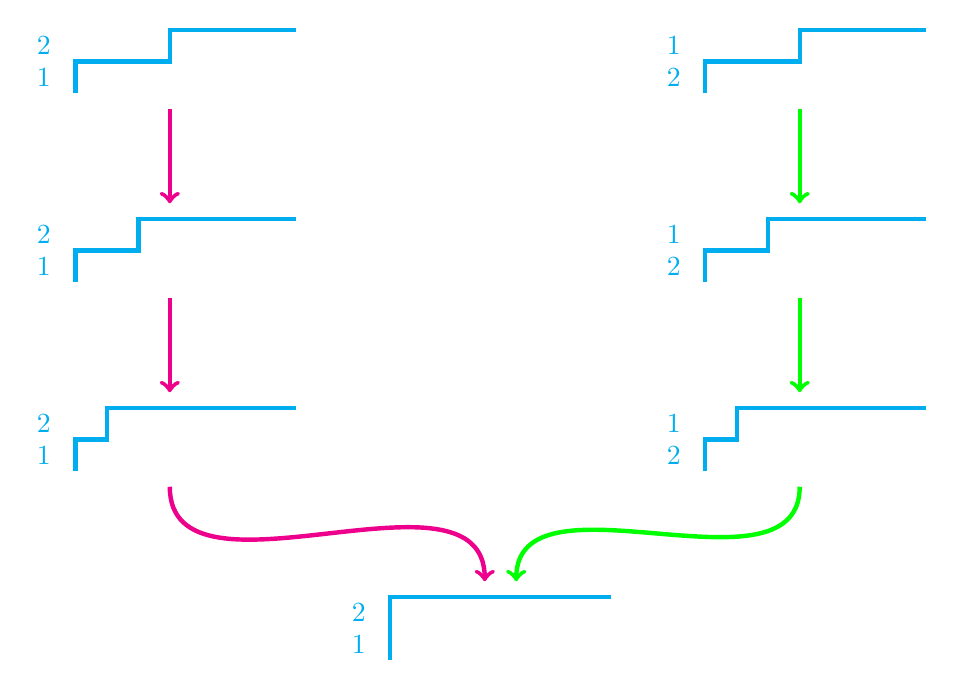
\begin{tikzpicture}[scale = 0.4]
            \draw [ultra thick, color = cyan] (0,0) -- (0,1)
                -- (0,2) -- (1,2) -- (2,2) -- (3,2) -- (4,2)
                -- (5,2) -- (6,2) -- (7,2);
            \node[color = cyan] at (-1,0.5) {$1$};
            \node[color = cyan] at (-1,1.5) {$2$};

            \draw [ultra thick, color = cyan] (-10,6) -- (-10,7)
                -- (-9,7) -- (-9,8) -- (-8,8) -- (-7,8)
                -- (-6,8) -- (-5,8) -- (-4,8) -- (-3,8);
            \node[color = cyan] at (-11,6.5) {$1$};
            \node[color = cyan] at (-11,7.5) {$2$};

            \draw [ultra thick, color = cyan] (10,6) -- (10,7)
                -- (11,7) -- (11,8) -- (12,8) -- (13,8)
                -- (14,8) -- (15,8) -- (16,8) -- (17,8);
            \node[color = cyan] at (9,6.5) {$2$};
            \node[color = cyan] at (9,7.5) {$1$};

            \draw [ultra thick, color = cyan] (-10,12) -- (-10,13)
                -- (-9,13) -- (-8,13) -- (-8,14) -- (-7,14)
                -- (-6,14) -- (-5,14) -- (-4,14) -- (-3,14);
            \node[color = cyan] at (-11,12.5) {$1$};
            \node[color = cyan] at (-11,13.5) {$2$};

            \draw [ultra thick, color = cyan] (10,12) -- (10,13)
                -- (11,13) -- (12,13) -- (12,14) -- (13,14)
                -- (14,14) -- (15,14) -- (16,14) -- (17,14);
            \node[color = cyan] at (9,12.5) {$2$};
            \node[color = cyan] at (9,13.5) {$1$};

            \draw [ultra thick, color = cyan] (-10,18) -- (-10,19)
                -- (-9,19) -- (-8,19) -- (-7,19) -- (-7,20)
                -- (-6,20) -- (-5,20) -- (-4,20) -- (-3,20);
            \node[color = cyan] at (-11,18.5) {$1$};
            \node[color = cyan] at (-11,19.5) {$2$};

            \draw [ultra thick, color = cyan] (10,18) -- (10,19)
                -- (11,19) -- (12,19) -- (13,19) -- (13,20)
                -- (14,20) -- (15,20) -- (16,20) -- (17,20);
            \node[color = cyan] at (9,18.5) {$2$};
            \node[color = cyan] at (9,19.5) {$1$};

            \draw [->][color=magenta, ultra thick]
                (-7,17.5) to (-7,14.5);
            \draw [->][color=magenta, ultra thick]
                (-7,11.5) to (-7,8.5);
            \draw [->][out=-90,in=90, ultra thick] 
                [color=magenta](-7,5.5) to (3,2.5);

            \draw [->][color=green, ultra thick]
                (13,17.5) to (13,14.5);
            \draw [->][color=green, ultra thick]
                (13,11.5) to (13,8.5);
            \draw [->][out=-90,in=90, ultra thick] 
                [color=green](13,5.5) to (4,2.5);
        
        \end{tikzpicture}
        ~\\
        ~\\
        There are $7^1 = 7$ elements in this poset.
    \end{center}
\end{example}

\begin{definition}[$\gtrdot$]
    For $f$ and $g$ two rational parking functions, we say
    that $f$ covers $g$, written $f \gtrdot g$, if
    $\exists i$ such that :
    \begin{itemize}
        \item $f = (a_1, \ldots, a_{i-1}, a_i,\ \ \ \ 
            a_{i+1}, \ldots, a_n)$
        \item $g = (a_1, \ldots, a_{i-1}, a_i - 1, a_{i+1},
        \ldots, a_n)$
    \end{itemize}
    That is, the same relation as for rational primitive
    parking functions.
\end{definition}

\begin{example}[$a > b : a = 7, b = 3$]
    $(2, 3, 1, 1, 2, 1, 3) \gtrdot (2, 3, 1, 1, 1, 1, 3)$    
\end{example}

\begin{example}[$a < b : a = 3, b = 5$]
    $(4, 1, 2) \gtrdot (3, 1, 2)$    
\end{example}

\begin{prop}
    This covering relation defines a \emph{poset}
    for $\mathcal{PF}_{a,b}$.
\end{prop}

\begin{example}[$a > b$ : The poset of $\mathcal{PF}_{5,2}$]
    ~\\
    \begin{center}
        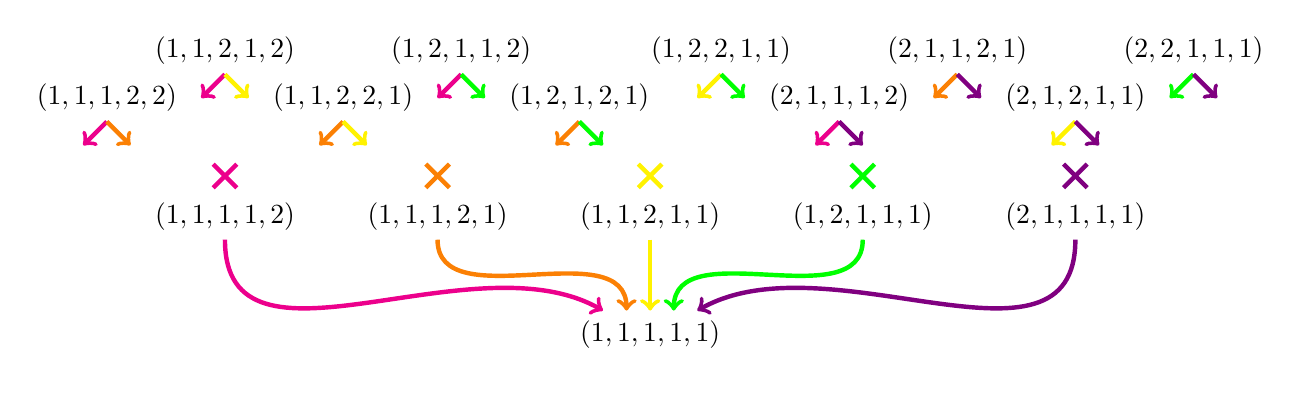
\begin{tikzpicture}[scale = 0.3]
            \node at (0,0) {$(1,1,1,1,1)$};

            \node at (-18,5) {$(1,1,1,1,2)$};
            \node at (-9,5)  {$(1,1,1,2,1)$};
            \node at (0,5)   {$(1,1,2,1,1)$};
            \node at (9,5)   {$(1,2,1,1,1)$};
            \node at (18,5)  {$(2,1,1,1,1)$};

            \node at (-23,10) {$(1,1,1,2,2)$};
            \node at (-18,12) {$(1,1,2,1,2)$};
            \node at (-13,10) {$(1,1,2,2,1)$};
            \node at (-8,12)  {$(1,2,1,1,2)$};
            \node at (-3,10)  {$(1,2,1,2,1)$};
            \node at (3,12)   {$(1,2,2,1,1)$};
            \node at (8,10)   {$(2,1,1,1,2)$};
            \node at (13,12)  {$(2,1,1,2,1)$};
            \node at (18,10)  {$(2,1,2,1,1)$};
            \node at (23,12)  {$(2,2,1,1,1)$};

            \draw [->][color=magenta, ultra thick]
                (-23,9) to (-24,8);
            \draw [->][color=magenta, ultra thick]
                (-18,11) to (-19,10);
            \draw [->][color=magenta, ultra thick]
                (-8,11) to (-9,10);
            \draw [->][color=magenta, ultra thick]
                (8,9) to (7,8);
            \draw[color=magenta, ultra thick]
                (-18.5,7.2) -- (-17.5,6.2);
            \draw[color=magenta, ultra thick]
                (-18.5,6.2) -- (-17.5,7.2);
            \draw [->][out=-90,in=150, ultra thick] 
                [color=magenta](-18,4) to (-2,1);

            \draw [->][color=brown!7!orange, ultra thick]
                (-23,9) to (-22,8);
            \draw [->][color=brown!7!orange, ultra thick]
                (-13,9) to (-14,8);
            \draw [->][color=brown!7!orange, ultra thick]
                (-3,9) to (-4,8);
            \draw [->][color=brown!7!orange, ultra thick]
                (13,11) to (12,10);
            \draw[color=brown!7!orange, ultra thick]
                (-9.5,7.2) -- (-8.5,6.2);
            \draw[color=brown!7!orange, ultra thick]
                (-9.5,6.2) -- (-8.5,7.2);
            \draw [->][out=-90,in=90, ultra thick]
                [color=brown!7!orange](-9,4) to (-1,1);

            \draw [->][color=yellow, ultra thick]
                (-18,11) to (-17,10); 
            \draw [->][color=yellow, ultra thick]
                (-13,9) to (-12,8); 
            \draw [->][color=yellow, ultra thick]
                (3,11) to (2,10); 
            \draw [->][color=yellow, ultra thick]
                (18,9) to (17,8); 
            \draw[color=yellow, ultra thick]
                (-0.5,7.2) -- (0.5,6.2);
            \draw[color=yellow, ultra thick]
                (-0.5,6.2) -- (0.5,7.2);
            \draw [->][out=-90,in=90, ultra thick] 
                [color=yellow](0,4) to (0,1);

            \draw [->][color = green,  ultra thick]
                (-8,11) to (-7,10);
            \draw [->][color=green, ultra thick]
                (-3,9) to (-2,8);
            \draw [->][color=green, ultra thick]
                (3,11) to (4,10);
            \draw [->][color=green, ultra thick]
                (23,11) to (22,10);
            \draw[color=green, ultra thick]
                (8.5,7.2) -- (9.5,6.2);
            \draw[color=green, ultra thick]
                (8.5,6.2) -- (9.5,7.2);
            \draw [->][out=-90,in=90, ultra thick]
                [color=green](9,4) to (1,1);

            \draw [->][color=violet, ultra thick]
                (8,9) to (9,8);
            \draw [->][color=violet, ultra thick]
                (13,11) to (14,10);
            \draw [->][color=violet, ultra thick]
                (18,9) to (19,8);
            \draw [->][color=violet, ultra thick]
                (23,11) to (24,10);
            \draw[color=violet, ultra thick]
                (17.5,7.2) -- (18.5,6.2);
            \draw[color=violet, ultra thick]
                (17.5,6.2) -- (18.5,7.2);
            \draw [->][out=-90,in=30, ultra thick] 
                [color=violet](18,4) to (2,1);
        
        \end{tikzpicture}
        ~\\
        ~\\
        Arrows have been simplified for readability.\\
        Arrows between the top 2 levels are to be read
        as ending at the cross of the corresponding color.\\
        There are $2^4 = 16$ elements in this poset.
    \end{center}
\end{example}

\begin{example}[$a < b$ : The poset of $\mathcal{PF}_{2,7}$]
    ~\\
    \begin{center}
        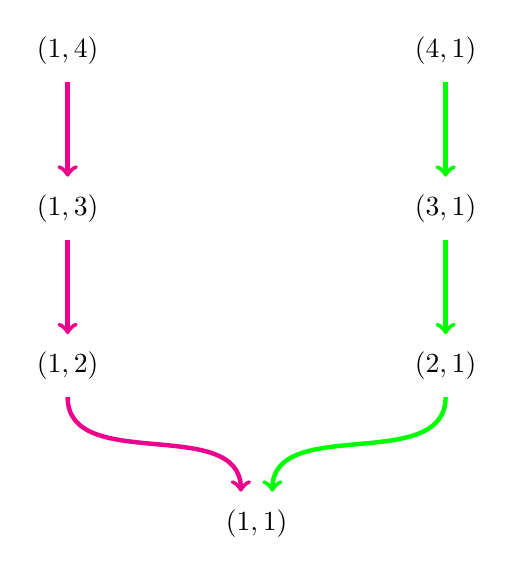
\begin{tikzpicture}[scale = 0.4]
            \node at (0,0) {$(1,1)$};

            \node at (-6,5) {$(1,2)$};
            \node at (6,5)  {$(2,1)$};

            \node at (-6,10) {$(1,3)$};
            \node at (6,10)  {$(3,1)$};

            \node at (-6,15) {$(1,4)$};
            \node at (6,15)  {$(4,1)$};

            \draw [->][color=magenta, ultra thick]
                (-6,14) to (-6,11);
            \draw [->][color=magenta, ultra thick]
                (-6,9) to (-6,6);
            \draw [->][out=-90,in=90, ultra thick] 
                [color=magenta](-6,4) to (-0.5,1);

            \draw [->][color=green, ultra thick]
                (6,14) to (6,11);
            \draw [->][color=green, ultra thick]
                (6,9) to (6,6);
            \draw [->][out=-90,in=90, ultra thick] 
                [color=green](6,4) to (0.5,1);
        
        \end{tikzpicture}
        ~\\
        ~\\
        There are $7^1 = 7$ elements in this poset.
    \end{center}
\end{example}

\begin{rem}
    The posets of $\mathcal{PF}_{a,b}$ and $\mathcal{LR}_{a,b}$
    are isomorphic, and one can be obtained by
    applying the aforementioned bijection to the other.
\end{rem}